% !TEX root = ../report/report.tex

%%%%%%%%%%%%%%%%%%%%%%%%%%%%%%%%%%%%%%%%%%%%%%%%%%%%%%%%%%%%
% EE227A Project: algorithms.tex
% Created by: Maximilian Balandat
% Last edited: Apr 02 2012
%%%%%%%%%%%%%%%%%%%%%%%%%%%%%%%%%%%%%%%%%%%%%%%%%%%%%%%%%%%%

% Use our own document class
%\documentclass{../../common/projectreport}

% Input some of my LaTeX macros - Max
%\newcommand{\norm}[3]{{\left\|#1\right\|}_{#2}^{#3}}
\newcommand{\normball}[2]{{\mathbb{B}_{#1}^{#2}}}
\newcommand{\proximal}[2]{{\prox_{#1}(#2)}}
\newcommand{\forAll}{{\forall \,}}
\newcommand{\Rbb}{{\mathbb R}}
\newcommand{\Rbf}{{\mathbf R}}
\newcommand{\Lhat}{{\hat{L}}}
\newcommand{\Shat}{{\hat{S}}}
\newcommand{\Yhat}{{\hat{Y}}}
\newcommand{\Xhat}{{\hat{X}}}
\newcommand{\Nbb}{{\mathbb N}}
\newcommand{\Fbb}{{\mathbb F}}
\newcommand{\Cbb}{{\mathbb C}}
\newcommand{\Tbb}{{\mathbb T}}
\newcommand{\Zbb}{{\mathbb Z}}
\newcommand{\etabar}{{\bar{\eta}}}
\newcommand{\kbar}{{\bar{k}}}
\newcommand{\rbar}{{\bar{r}}}
\newcommand{\xibar}{{\bar{\xi}}}
\newcommand{\ubar}{{\bar{u}}}
\newcommand{\vbar}{{\bar{v}}}
\newcommand{\uhat}{{\hat{u}}}
\newcommand{\vbf}{{\mathbf{v}}}
\newcommand{\vhat}{{\hat{v}}}
\newcommand{\xbar}{{\bar{x}}}
\newcommand{\xhat}{{\hat{x}}}
\newcommand{\xdot}{{\dot{x}}}
\newcommand{\Xdot}{{\dot{X}}}
\newcommand{\xtilde}{{\tilde{x}}}
\newcommand{\xtildedot}{{\dot{\tilde{x}}}}
\newcommand{\Phitilde}{{\tilde{\Phi}}}
\newcommand{\phat}{{\hat{p}}}
\newcommand{\shat}{{\hat{s}}}
\newcommand{\xbf}{{\mathbf{x}}}
\newcommand{\wbf}{{\mathbf{w}}}
\newcommand{\Pbf}{{\mathbf{P}}}
\newcommand{\Xbf}{{\mathbf{X}}}
\newcommand{\Ebf}{{\mathbf{E}}}
\newcommand{\Obf}{{\mathbf{0}}}
\newcommand{\ebf}{{\mathbf{e}}}
\newcommand{\alphabf}{{\mathbf{\alpha}}} 
\newcommand{\alphabar}{{\bar{\alpha}}} 
\newcommand{\sgn}{\text{sgn}}
\newcommand{\Range}{\mathcal{R}}
\newcommand{\Nullspace}{\mathcal{N}}

\newcommand{\pderiv}[2]{\frac{\partial #1}{\partial #2}}
\newcommand{\pderivsq}[2]{\frac{\partial^2 #1}{\partial #2^2}}
\newcommand{\pderivxy}[3]{\frac{\partial^2 #1}{\partial #2 \partial #3}}

\newcommand{\One}{{\mathbf{1}}}

\newcommand{\Ccal}{{\mathcal{C}}}
\newcommand{\Dcal}{{\mathcal{D}}}
\newcommand{\Fcal}{{\mathcal{F}}}
\newcommand{\Hcal}{{\mathcal{H}}}
\newcommand{\Lcal}{{\mathcal{L}}}
\newcommand{\Ncal}{{\mathcal{N}}}
\newcommand{\Pcal}{{\mathcal{P}}}
\newcommand{\Qcal}{{\mathcal{Q}}}
\newcommand{\Rcal}{{\mathcal{R}}}
\newcommand{\Scal}{{\mathcal{S}}}
\newcommand{\Tcal}{{\mathcal{T}}}
\newcommand{\Ucal}{{\mathcal{U}}}
\newcommand{\Xcal}{{\mathcal{X}}}
\newcommand{\Ycal}{{\mathcal{Y}}}


\newcommand{\ifthen}[2]{\textbf{if} #1 \textbf{then} #2}
\newcommand{\ifthenreturn}[2]{\textbf{if} #1 \textbf{then return} #2}
\newcommand{\then}[1]{\textbf{then} #1}
\newcommand{\return}[1]{\textbf{return} #1}
\newcommand{\returns}[1]{\textbf{returns} #1}
\newcommand{\thenreturn}[1]{\textbf{then return} #1}
\newcommand{\foreachindo}[3]{\textbf{for each} #1 \textbf{in} #2 \textbf{do} #3}
\newcommand{\algindent}[1]{\STATE\hspace{#1\algorithmicindent}}

\DeclareMathOperator{\blkdiag}{blkdiag}
\DeclareMathOperator{\trace}{\mathbf{Tr}}
\DeclareMathOperator{\Convh}{Conv}
\DeclareMathOperator{\rank}{rk}
\DeclareMathOperator{\diag}{diag}
\DeclareMathOperator{\Realpart}{Re}
\DeclareMathOperator{\Imagpart}{Im}
\DeclareMathOperator{\Poles}{Poles}
\DeclareMathOperator{\spanspace}{span}
\DeclareMathOperator*{\argmax}{arg\,max}
\DeclareMathOperator*{\argmin}{arg\,min}
\DeclareMathOperator{\Onebf}{{\mathbf{1}}}
\DeclareMathOperator{\dom}{dom}
\DeclareMathOperator{\grad}{\nabla\!\!}
\DeclareMathOperator{\epi}{epi}
\DeclareMathOperator{\sign}{sign}
\DeclareMathOperator{\divergence}{div}
\DeclareMathOperator{\prox}{prox}

\newcommand\independent{\protect\mathpalette{\protect\independenT}{\perp}}
\def\independenT#1#2{\mathrel{\rlap{$#1#2$}\mkern2mu{#1#2}}}


\newcommand{\Acal}{{\mathcal{A}}}
\newcommand{\Abar}{{\bar{A}}}


\theoremstyle{plain}
\newtheorem{thm}{Theorem}
\theoremstyle{plain}
\newtheorem{fact}[thm]{Fact}
\theoremstyle{plain}
\newtheorem{prop}[thm]{Proposition}




%%%%%%%%%%%%%%%%%%%%%%%%%%%%%%%%%%%%%%%%%%%%%%%%%%%%%%%%%%%%
%\begin{document}


%%%%%%%%%%%%%%%%%%%%%%%%%%%%%%%%%%%%%%%%%%%%
\section{Overview}
\label{Algorithms:Overview:Sec}

This section discusses some of the algorithms that have recently been proposed in the literature to solve the Robust PCA problem
%
\begin{align}
\begin{split}
p^* = \min_{L,S} \; &\norm{L}{*}{} + \lambda \norm{S}{1}{} \\
\text{s.t.} \quad &M = L+S
\end{split}
\label{Algorithms:Overview:RecallRPCA}
\end{align}

There are various methods that can be used to solve~\eqref{Algorithms:Overview:RecallRPCA}. A straightforward way described in section~\ref{Algorithms:MainAlgs:IPM:Subsec} is to use general purpose interior point solvers~\cite{Sturm:1999uq,Toh:1999kx} to solve an SDP formulation of the dual of~\eqref{Algorithms:Overview:RecallRPCA}, an approach that works well for low-dimensional data~$M$ but unfortunately does not scale well. Another approach is to use iterative thresholding techniques as described in section~\ref{Algorithms:MainAlgs:ITM:Subsec}, which result in a very simple algorithm that can be applied also to high-dimensional data. Unfortunately the convergence of this algorithm is extremely slow. More sophisticated approaches include an accelerated proximal gradient algorithm (section~\ref{Algorithms:MainAlgs:PGM:Subsec}) and a gradient ascent algorithm applied to the dual problem of~\eqref{Algorithms:Overview:RecallRPCA} (section~\ref{Algorithms:MainAlgs:GAD:Subsec}). The current state of the art seems to be a adaptation of the Augmented Lagrangian Method to the non-smooth problem~\eqref{Algorithms:Overview:RecallRPCA}, an approach that is discussed in section~\ref{Algorithms:MainAlgs:AugLag:Subsec}.



%%%%%%%%%%%%%%%%%%%%%%%%%%%%%%%%%%%%%%%%%%%%
\section{Main algorithms for Robust PCA}
\label{Algorithms:MainAlgs:Sec}

%This section reviews a number of different approaches to solving the Robust PCA problem. 

%%%%%%%%%%%%%%%%%%%%%%%%%%%%
\subsection{Interior Point Methods}
\label{Algorithms:MainAlgs:IPM:Subsec}

As will be shown in the following section, the dual problem of~\eqref{Algorithms:Overview:RecallRPCA} can be cast as a Semidefinite Programming (SDP) problem for which a number of efficient polynomial-time interior-point solvers have been developed. In principle, one can then just apply these general purpose off-the-shelf solvers to the dual SDP. This approach will work well for small and medium sized problems, but unfortunately it does not scale with the size of the data matrix~$M$. The following section first develops the dual of the Robust PCA problem, section~\ref{Algorithms:MainAlgs:IPM:Complexity:Subsubsec} then discusses the limitations of using interior point methods on the resulting SDP. 


%%%%%%%%%%%%%%%%%
\subsubsection{Formulation of the Dual problem of Robust PCA as an SDP}
\label{Algorithms:MainAlgs:IPM:SDPform:Subsubsec}

Let us use the equality constraint to eliminate the variable~$L$ from~\eqref{Algorithms:Overview:RecallRPCA}. Using the facts that $\norm{X}{*}{} = \max_{\norm{Y}{2}{}\leq 1} \trace Y^T\!X$ and $\norm{X}{1}{} = \max_{\norm{Z}{\infty}{}\leq 1} \trace Z^T\!X$  the problem can be written as
%
\begin{align}
\begin{split}
p^* = \min_S \;\max_{Y,Z} \;\; &\trace Y^T(M-S) + \lambda \trace Z^TS \\
\text{s.t.} \quad & \norm{Y}{2}{}\leq 1 \\
&\norm{Z}{\infty}{}\leq 1
\end{split}
\label{Algorithms:MainAlgs:IPM:SDPform:NoNorms}
\end{align}
%
The dual function is 
\begin{align}
\begin{split}
g(Y,Z) &= \min_S \;\; \trace Y^T\!M + \trace (\lambda Z-Y)^T\!S \\
&= \begin{cases}
\trace Y^T\!M  & \text{ if } \; \lambda Z = Y \\
-\infty & \text{ otherwise }
\end{cases} 
\end{split}
\label{Algorithms:MainAlgs:IPM:SDPform:DualFunct}
\end{align}
%
We obtain the dual problem 
\begin{align}
\begin{split}
p^* \geq d^* = \max_{Y,Z} \;\; &\trace Y^T\!M \\
\text{s.t.} \quad & \lambda Z = Y \\
&\norm{Y}{2}{}\leq 1 \\
&\norm{Z}{\infty}{}\leq 1
\end{split}
\label{Algorithms:MainAlgs:IPM:SDPform:DualProb}
\end{align}
%
which after eliminating the variable~$Z$ and using homogeneity of the norm becomes
\begin{align}
\begin{split}
d^* = \max_{Y} \;\; &\trace Y^T\!M \\
\text{s.t.} \quad & \norm{Y}{2}{}\leq 1 \\
&\norm{Y}{\infty}{}\leq \lambda
\end{split}
\label{Algorithms:MainAlgs:IPM:SDPform:DualSimpler}
\end{align}

Noting that $\norm{Y}{2}{}\leq 1 \; \Longleftrightarrow \; I-X^T(I)^{-1}X \succeq 0$ and using a Schur Complement lemma, the dual problem can be transformed into the following SDP standard form:
\begin{align}
\begin{split}
d^* = \max_{Y} \;\; &\trace M^T\!Y \\ 
\text{s.t.} \quad &\begin{bmatrix} I & Y^T \\ Y & I \end{bmatrix} \succeq 0 \\
&\trace \Delta_{ij}^TY \leq \lambda, \quad i = 1,\dotsc, m, \; j=1,\dotsc,n \\
&\trace \Delta_{ij}^TY \geq -\lambda, \quad i = 1,\dotsc, m, \; j=1,\dotsc,n
\end{split}
\label{Algorithms:MainAlgs:IPM:SDPform:DualSDP}
\end{align}
%
Here $\Delta_{ij} \in \Rbf^{m\times n}$ is such that $\Delta_{ij}(k,l) = \delta_{ik}\delta_{jl}$. Note that both primal and dual problem are (trivially) strictly feasible. In fact, the primal is unconstrained and an obvious strictly feasible dual variable is~$Y=0$. Hence strong duality holds ($p^* = d^*$) and both primal and dual problem are attained.\\

\textbf{Recovering the primal solution}

To recover the primal solution we can distinguish the two cases $\lambda \leq 1$ and $\lambda >1$. For the latter one, first note that $\norm{Y}{\infty}{} \leq \norm{Y}{2}{}$ for all~$Y$. To show this first recall that $c := \norm{Y}{2}{} = \max_{\norm{x}{2}{}=1} \norm{Yx}{2}{}$. This means that $c - x^TY^TYx \geq0, \,\forAll x$ or, equivalently, $cI-Y^TY \succeq 0$. Using a Schur Complement this can be written as
%
\begin{align*}
\begin{bmatrix} I & Y \\Y^T & cI \end{bmatrix} \succeq 0
\end{align*}
It is easy to see that this implies that  
\begin{align*}
\begin{bmatrix} 1 & Y_{ij} \\Y_{ij} & c \end{bmatrix} \succeq 0
\end{align*}
for all $i,j$, which is equivalent to $|Y_{ij}| \leq c,\; \forAll i,j$. This shows that $\norm{Y}{\infty}{} \leq \norm{Y}{2}{}$.

Hence we observe that if $\lambda >1$ the constraint $\norm{Y}{2}{} \leq \lambda$ will be inactive, that is $|Y_{ij}|<\lambda,\;\forAll i,j$. Therefore, for $\lambda > 1$, removing this constraint from~\eqref{Algorithms:MainAlgs:IPM:SDPform:DualSimpler} does not change the problem. We have $d^* = \max_{\norm{Y}{2}{}\leq 1} \trace Y^T\!M = \norm{M}{*}{}$, and this lower bound is achieved by the primal (feasible) solution $L=M$ and $S =0$.

If $\lambda \leq 1$, then we can look at the dual of the dual~\eqref{Algorithms:MainAlgs:IPM:SDPform:DualSimpler}. One way to form a Lagrangian of this dual problem is to introduce Lagrange multipliers $S_- \geq 0$ and $S_+ \geq 0$ for the constraints $Y_{ij} \leq \lambda$ and $-Y_{ij} \leq \lambda$, respectively:
\begin{align*}
\mathcal{L}(Y, S_+, S_-) 
&= -\trace Y^T M - \trace S_-^T(Y - \lambda 1) - \trace S_+^T(-Y - \lambda 1) \\
&= \trace (S_+ - S_- - M)^T Y + \lambda \trace (S_+ + S_-)^T 1
\end{align*}
Here $1$ denotes the $n \times n$ matrix whose entries are all ones. We have
\begin{align*}
d^*
&= \max_{\substack{\|Y\|_2 \leq 1 \\ \|Y\|_\infty \leq \lambda}}\; -\trace M^T Y\\
&= \max_{\|Y\|_2 \leq 1}\; \min_{\substack{S_+ \geq 0 \\ S_- \geq 0}}\; \mathcal{L}(Y, S_+, S_-) \\
&= \min_{\substack{S_+ \geq 0 \\ S_- \geq 0}}\; \max_{\|Y\|_2 \leq 1}\;  \mathcal{L}(Y, S_+, S_-) \\
&= \min_{\substack{S_+ \geq 0 \\ S_- \geq 0}}\; g(S_+, S_-)
\end{align*}
where 
\begin{align*}
g(S_+, S_-) 
&= \max_{\|Y\|_2 \leq 1} \trace (S_+ - S_- - M)^T Y + \lambda \trace (S_+ + S_-)^T 1 \\
&= \|S_+ - S_- - M\|_* + \lambda \trace (S_+ + S_-)^T 1
\end{align*}
A dual problem of the dual~\eqref{Algorithms:MainAlgs:IPM:SDPform:DualSimpler} is then simply
\begin{align}
&\min_{S_+\geq 0, S_-\geq 0}\; \|S_+ - S_- - M\|_* + \lambda \trace (S_+ + S_-)^T 1
\end{align}


We have $d^* = \min_{S_+\geq 0, S_-\geq 0} g(S_+, S_-)$. Note that at the optimum, the variables $S_+$ and $S_-$ satisfy $\min (S_{+ij}, S_{-ij}) = 0$ $\forall i,j$. Indeed, suppose there existed $(i,j)$ such that $\min(S_{+ij}, S_{-ij}) = a > 0$, then $g(S_+ - ae_ie_j^T, S_- - ae_ie_j^T) = g(S_+, S_-) - 2\lambda a < g(S_+, S_-)$, and $(S_+, S_-)$ is not optimal. Letting $S = S_+ - S_-$, the problem is equivalent to the primal~
\begin{align*}
p^* = \min_{S} \; &\norm{M-S}{*}{} + \lambda \norm{S}{1}{} 
\end{align*}
Therefore it is possible to recover the optimizer $S^*$ from the dual problem: Indeed, we have that $S^* = S_+^* - S_-^*$ where $S_-$ and $S_+$ are respectively the Lagrange multipliers associated with the constraints $Y_{ij} \leq \lambda$ and $-Y_{ij} \leq \lambda$



%%%%%%%%%%%%%%%%%
\subsubsection{Using Interior Point Methods to Solve the Dual}
\label{Algorithms:MainAlgs:IPM:Complexity:Subsubsec}

Problem~\eqref{Algorithms:MainAlgs:IPM:SDPform:DualSimpler} is an SDP and can therefore in principle be solved using off-the-shelf solver packages such as \texttt{sedum}~\cite{Sturm:1999uq} and \texttt{sdpt3}~\cite{Toh:1999kx}. These solvers are based on interior point methods which offer superior convergence rates~\cite{Boyd:2004aa} but unfortunately do not scale ell at all with the size of the matrix~$M$. Figure~\ref{Algorithms:MainAlgs:IPM:Complexity:figure} shows the average running time over 10 instances of the dual problem for the solvers \texttt{sedumi} and \texttt{sdpt3} for randomly generated data of very low dimensions. 
%
\begin{figure}[htbp]
\centering
\includegraphics[width=0.5\textwidth]{../figures/intpt_comparison}
\caption{Average running time of interior point methods for the dual problem}
\label{Algorithms:MainAlgs:IPM:Complexity:figure}
\end{figure}
%
There is a surprisingly big difference in terms of the running times: \texttt{sdpt3} is consistently faster than \texttt{sedumi}, with the spread growing significantly with the problem size. For the largest dimension \texttt{sdpt3} on average is 8 times faster than \texttt{sedumi} for this particular problem type. To be able to give a realistic assessment of why this is the case would however require detailed knowledge of the solver implementation. 

Regardless of which solver is used, it is obvious that, with an average running time of the faster of the two solvers of more than 2 minutes even on toy-sized problems involving matrices with only 2500 entries, interior point solvers are unsuitable for most problem of interest. The reason for this extremely bad scaling behavior with the matrix dimension is that the computation of the Newton step direction relies on second-order information of the (barrier-augmented) objective function, the computation of which is infeasible when the number of variables is very high. For applications that involve large-scale data matrices (with~$mn$ in the millions or even billions), using interior point methods therefore is essentially impossible. In order to overcome this scalability issue, a variety of first-order methods exploiting the particular structure of the Robust PCA problem have been proposed. Some of these methods will be described in the following.


%%%%%%%%%%%%%%%%%%%%%%%%%%%%
\subsection{Iterative Thresholding Method}
\label{Algorithms:MainAlgs:ITM:Subsec}

Among the first techniques used to solve~\eqref{Algorithms:Overview:RecallRPCA} for high-dimensional data was an adaptation \cite{Wright:2009fk}\footnote{note that the iterative thresholding algorithm seems to never have appeared in the published version of~\cite{Wright:2009fk}, which instead contains the accelerated proximal gradient method described in section~\ref{Algorithms:MainAlgs:PGM:Subsec}} of an iterative thresholding method originally proposed for the matrix completion problem in~\cite{Cai:2010uq}. For this method the authors of consider a relaxation of the original problem~\eqref{Algorithms:Overview:RecallRPCA} of the form 
%
\begin{align}
\begin{split}
\min_{L,S} \;\; &\norm{L}{*}{} + \lambda \norm{S}{1}{} + \frac{1}{2\tau} \norm{L}{F}{2} + \frac{1}{2\tau} \norm{S}{F}{2} \\
\text{s.t.} \quad &M=L+S
\end{split}
\label{Algorithms:MainAlgs:ITM:Relax}
\end{align}
%
where $\tau \gg 1$ is a scalar parameter. Generalizing the result from~\cite{Cai:2010uq} (which considers the matrix completion problem, i.e. $S=0$), the authors of~\cite{Wright:2009fk} argue that for large values of~$\tau$ the solution of~\eqref{Algorithms:MainAlgs:ITM:Relax} will be very close to that of~\eqref{Algorithms:Overview:RecallRPCA}. One can now employ iterative thresholding techniques to solve~\eqref{Algorithms:MainAlgs:ITM:Relax}. Although the resulting algorithm has little relevance in practice because of its extremely slow convergence speed, we will see in the following sections that its main ideas are the basis for a number of other similar algorithms. Therefore we briefly review the iterative thresholding algorithm here.\\ 

The Lagrangian of the problem~\eqref{Algorithms:MainAlgs:ITM:Relax} is given by
%
\begin{align}
\Lcal(L,S,Y) = \norm{L}{*}{} + \lambda \norm{S}{1}{} + \frac{1}{2\tau} \norm{L}{F}{2} + \frac{1}{2\tau} \norm{S}{F}{2} + \frac{1}{\tau} \langle Y, M-L-S \rangle
\label{Algorithms:MainAlgs:ITM:Lagr}
\end{align}
%
The idea of the iterative thresholding algorithm is, as the name suggests, to update the variables $L,S$ and $Y$ iteratively. More specifically, the Lagrangian $\Lcal(L,S,Y)$ is minimized w.r.t $L$ and $S$ for some fixed dual variable~$Y$, and the violation of the constraint is then used to update~$Y$ using the gradient step~$Y^+ = Y + t (M-L-S)$, where~$0<t<1$ is the step size.\\

Note that for fixed~$Y$ we have
%
\begin{align}
\begin{split}
(\Lhat,\Shat) :&= \argmin_{L,S} \; \Lcal(L,S,Y) \\
&= \argmin_{L,S} \; \norm{L}{*}{} + \lambda \norm{S}{1}{} + \frac{1}{2\tau} \norm{L}{F}{2} + \frac{1}{2\tau} \norm{S}{F}{2} + \frac{1}{\tau} \langle Y, M-L-S \rangle \\
&= \argmin_{L,S} \; \norm{L}{*}{} + \lambda \norm{S}{1}{} + \frac{1}{2\tau} \norm{L-Y}{F}{2} + \frac{1}{2\tau} \norm{S-Y}{F}{2}
\end{split}
\label{Algorithms:MainAlgs:ITM:ArgminLagr}
\end{align}
%
We note that the above problem is completely separable hence the minimizers~$\Lhat$ and~$\Shat$ can be determined independently. Using optimality conditions based on the subgradient it can be shown~\cite{Cai:2010uq,Wright:2009fk} that the minimizers~$\Lhat$ and~$\Shat$ are both of a simple form. To this end, consider the following 
% where~$\Scal_\varepsilon[X]$ is the 
extension to the matrix case of the well known soft-thresholding operator (e.g. from the proximal mapping of the~$l_1$-norm in the vector case):
%
\begin{align}
\left(\Scal_\varepsilon[X]\right)_{ij} := \begin{cases} x_{ij}-\varepsilon & \text{ if} \;\; x_{ij}>\varepsilon \\ x_{ij}+\varepsilon & \text{ if} \;\; x_{ij}<-\varepsilon \\ 0 & \text{ otherwise} \end{cases}
\label{Algorithms:MainAlgs:ITM:Shrink}
\end{align}


\begin{theorem}[Singular Value Thresholding~\cite{Cai:2010uq}]
For each $\tau \geq 0$ and $Y\in \Rbf^{m\times n}$, we have that
\begin{align}
\Dcal_\tau(Y) := U \Scal_\tau[\Sigma] V^T = \argmin_X \; \norm{X}{*}{} + \frac{1}{2\tau} \norm{X-Y}{F}{2}
\label{Algorithms:MainAlgs:ITM:SVTtheore:eq}
\end{align}
where $Y = U\Sigma V^*$ is the SVD of~$Y$.
\label{Algorithms:MainAlgs:ITM:SVTtheorem}
\end{theorem}

Since Theorem~\ref{Algorithms:MainAlgs:ITM:SVTtheorem} is of fundamental importance to all algorithms discussed in this chapter, we give its proof here.
%
\begin{proof}[Proof of Theorem~\ref{Algorithms:MainAlgs:ITM:SVTtheorem}] 
Since the objective function $f_0(X) := \argmin_X \; \norm{X}{*}{} + \frac{1}{2\tau} \norm{X-Y}{F}{2}$ is strictly convex its minimizer is unique. Recall that $Z$ is a subgradient of a convex function $f:\Rbf^{m\times n} \mapsto \Rbf$ at $X_0$ if $f(X) \geq f(X_0) + \langle Z,X-X_0\rangle$ for all~$X$. The set of all sugradients~$Z$ at $X_0$ is called the subdifferential and denoted $\partial f(X_0)$. By definition it follows that $\Xhat$ minimizes $f_0$ if and only if $0$ is as subgradient of $f_0$ at $\Xhat$. Using standard subgradient calculus this translates to $0 \in \Xhat - Y + \tau \partial ||\Xhat||_{*}$, where $\partial ||\Xhat||_{*}$ is the subdifferential of the nuclear norm at $\Xhat$. To show that $\Dcal_\tau(Y)$ satisfies~\eqref{Algorithms:MainAlgs:ITM:SVTtheore:eq} we therefore need to show that $0 \in \Dcal_\tau(Y)  - Y + \tau \partial ||\Dcal_\tau(Y) ||_{*}$.  

Let $X\in \Rbf^{m\times n}$ be arbitrary Let $U\Sigma V^*$ be its SVD. It can be shown that 
\begin{align*}
\partial ||X||_{*} = \left\{ UV^*+W \,\mid\, W\in \Rbf^{m\times n},\; U^*W =0,\; WV =0,\; \norm{W}{2}{}\leq 1 \right\}
\end{align*}
To use the above result decompose the SVD of~$Y$ as $Y = U_0\Sigma_0V_0^* + U_1\Sigma_1V_1^*$, where $U_0,V_0$ ($U_1,V_1$) are the singular vectors associated with singular values greater (less or equal) than~$\tau$. With this notation we have $\Dcal_\tau(Y) = U_0(\Sigma_0-\tau I)V_0^*$,  so $Y-\Dcal_\tau(Y) = \tau (U_0V_0^*+W)$ with $W=\tau^{-1}U_1\Sigma_1V_1^*$. By definition of the SVD $U_0^*W=0$ and $WV_0=0$. Furthermore, since $\max(\Sigma_1) \leq \tau$ it also holds that $\norm{W}{2}{}\leq 1$. Together this shows that $Y - \Dcal_\tau(Y) \in \tau \partial ||\Dcal_\tau(Y) ||_{*}$.
\end{proof}


It is also not hard to find the minimizer~$\Shat$ of~\eqref{Algorithms:MainAlgs:ITM:Lagr}, as the following proposition shows:\\

\begin{proposition}[Matrix Value Thresholding]
For each $\tau,\lambda \geq 0$ and $Y\in \Rbf^{m\times n}$, we have that
\begin{align}
\Scal_{\tau\lambda}[Y] = \argmin_X \; \lambda \norm{X}{1}{} + \frac{1}{2\tau} \norm{X-Y}{F}{2}
\label{Algorithms:MainAlgs:ITM:MVTprop:eq}
\end{align}
\label{Algorithms:MainAlgs:ITM:MVTprop}
\end{proposition}
%
\begin{proof}[Proof of Proposition~\ref{Algorithms:MainAlgs:ITM:MVTprop}] 
Note that the objective function $h_0(X) := \lambda \norm{X}{1}{} + \frac{1}{2\tau} \norm{X\!-\!Y}{F}{2}$ in~\eqref{Algorithms:MainAlgs:ITM:MVTprop:eq} is completely decomposable and can be written in the form $h_0(X) = \sum_{i,j} \lambda |X_{ij}| + \frac{1}{2\tau} (X_{ij}\!-\!Y_{ij})^2$, so the minimization over $X$ can be carried out element-wise. Using the same reasoning as in the proof of Theorem~\ref{Algorithms:MainAlgs:ITM:SVTtheorem}, we have that the element $X_{ij}$ is a minimizer if and only if $0 \in \partial h_0(X)$. This condition can be written as $Y_{ij}-X_{ij} \in \tau \lambda\, \partial |X_{ij}|$. We consider the cases $X_{ij} =0$ and $X_{ij} \neq 0$. If $X_{ij} =0$ then the condition reads $Y_{ij} \in \tau \gamma [-1,1]$. In other words, when $|Y_{ij}| \leq \tau \gamma$ then $X_{ij}=0$. On the other hand, if $X_{ij} \neq 0$, then  $\partial \, |X_{ij}| = \sign(X_{ij})$ and we have $X_{ij}= Y_{ij} -\tau\lambda \sign(Y_{ij})$, which is in fact the soft-thresholding operator $\Scal_{\tau\lambda}[X_{ij}]$.
\end{proof}


Applying Theorem~\ref{Algorithms:MainAlgs:ITM:SVTtheorem} and Proposition~\ref{Algorithms:MainAlgs:ITM:MVTprop} to~\eqref{Algorithms:MainAlgs:ITM:ArgminLagr} we find that the minimizers~$\Lhat$ and~$\Shat$ of~\eqref{Algorithms:MainAlgs:ITM:Lagr} are given, respectively, by 
%
\begin{align}
\Lhat &= U \Scal_\tau[\Sigma] V^T
\label{Algorithms:MainAlgs:ITM:ArgminLhat} \\
\Shat &= \Scal_{\tau\lambda}[Y]
\label{Algorithms:MainAlgs:ITM:ArgminShat}
\end{align}
%
%
Algorithm~\ref{Algorithms:MainAlgs:ITM:Algorithm} summarizes the overall iterative thresholding algorithm for Robust PCA. 
%
\begin{algorithm}
\caption{Iterative Thresholding Algorithm}
\KwIn{Observation matrix~$M$, parameters~$\lambda,\tau$}
initialization: $k=0$, $Y_0 = 0$\;
\While{not converged}{
$k=k+1$\;
$(U,\Sigma,V) = \text{svd}(Y_{k-1})$\;
$L_k = U \Scal_\tau[\Sigma] V^T$\;
$S_k = \Scal_{\lambda\tau}[Y_{k-1}]$\;
$Y_k = Y_{k-1} + t_k (M-L_k-S_k)$\;
}
\KwOut{$L=L_k$, $S=S_k$}
\label{Algorithms:MainAlgs:ITM:Algorithm}
\end{algorithm}

Algorithm~\ref{Algorithms:MainAlgs:ITM:Algorithm} is extremely simple to implement, as each iteration only requires the computation of an SVD of the current dual variable~$Y_k$ and a few elementary matrix operations. Note that, in fact, since the shrinking operator sets all singular values less than the threshold parameter to zero one really only needs to compute the singular values that lie above this threshold. In section~\ref{Algorithms:Discussion:SVD:PartialSVD:Subsubsec} we will discuss how this can be exploited to achieve potential speedups in all of the algorithms considered in this chapter. The convergence criterion used in practice is usually of the form $\|M-L_k-S_k\|_F < \varepsilon \norm{M}{F}{}$, where~$\varepsilon$ is the desired relative accuracy. 

While the iterative thresholding scheme in Algorithm~\ref{Algorithms:MainAlgs:ITM:Algorithm} is very simple and has been proved to converge, its convergence speed unfortunately is extremely slow. The authors of~\cite{Wright:2009fk} found that it typically requires about~$10^4$ iterations to converge for problems of reasonable size, an observation that is confirmed by our numerical experiments. Furthermore it is hard to find good general schemes to optimize the choice of the step size~$t_k$~\cite{Lin:2010fk}. As it turns out the other algorithms discussed in the following sections have a comparable complexity but converge much faster, both in theory and practice. Therefore the practical applicability of this approach is limited.


%%%%%%%%%%%%%%%%%%%%%%%%%%%%
\subsection{Accelerated Proximal Gradient Method}
\label{Algorithms:MainAlgs:PGM:Subsec}

An accelerated proximal gradient (APG) method for solving~\eqref{Algorithms:Overview:RecallRPCA} was proposed in~\cite{Lin:2009kx}. The method is essentially an application of the FISTA algorithm~\cite{Beck:2009kx} to a relaxation of the original RPCA problem in combination with a continuation technique. This FISTA algorithm algorithm is reminiscent of Nesterov's ``optimal'' first-oder method for smooth objective functions~\cite{Nesterov:1983uq}, whose~$O(1/\varepsilon)$ convergence result was extended to non-smooth objectives in~\cite{Nesterov:2007kx}. Besides being theoretically appealing, the APG method is also in practice much faster than the iterative thresholding algorithm discussed in section~\ref{Algorithms:MainAlgs:ITM:Subsec}.\\

The following sections describe the APG algorithm. As in~\cite{Lin:2009kx} we first give a general formulation and then show how it can be applied to the Robust PCA problem, using ideas from section~\ref{Algorithms:MainAlgs:ITM:Subsec}.


%%%%%%%%%%%%%%%%%
\subsubsection{A General Form of the Accelerated Proximal Gradient Method}
\label{Algorithms:MainAlgs:PGM:General:Subsubsec}

Proximal gradient algorithms in general can be used to solve unconstrained problems of the form 
%
\begin{align}
\min_{x} \;\; &f(x) := g(x) + h(x)
\label{Algorithms:MainAlgs:PGM:General:GenPGA}
\end{align}
%
where~$g$ is convex and differentiable and~$h$ is closed\footnote{that is, its epigraph is closed}, convex but need not be differentiable. The proximal mapping of a convex function~$h$ is defined as
%
\begin{align}
\proximal{h}{x} := \argmin_u \left( h(u) + \frac{1}{2}\norm{u-x}{}{2} \right)
\label{Algorithms:MainAlgs:PGM:General:proxmapping}
\end{align}
%
Here $\norm{\cdot}{}{}$ denotes the inner product norm\footnote{the derivation holds for real inner product spaces, not just~$\Rbf^n$. We are particularly interested in the case~$\Rbf^{m\times n}$}. Note that since~$h$ is convex and the norm is strictly convex, the optimizer in~\eqref{Algorithms:MainAlgs:PGM:General:proxmapping} is unique. The step of each iteration of the classic (non-accelerated) proximal gradient algorithm is
%
\begin{align}
x^+ = \proximal{\delta h}{x-\delta \nabla g(x)}
\label{Algorithms:MainAlgs:PGM:General:proxAlg}
\end{align}
%
where~$x^+$ denotes the next iterate, based on the current iterate~$x$, and~$\delta$ is the step size (which can be fixed or determined via backtracking line search). Since the proximal mapping~\eqref{Algorithms:MainAlgs:PGM:General:proxAlg} needs to be computed at each iteration (possibly multiple times because of the line search), the algorithm is most effective when this can be done cheaply. Depending on the function~$h$, the proximal gradient algorithm can be seen as a generalization of different gradient-based algorithms. In particular, for~$h(x) \equiv 0$ the standard gradient algorithm is recovered and for~$h(x) = I_C(x)$, where $I_C$ denotes the indicator function for the convex set~$C$, the projected gradient algorithm is recovered. 

Note that~\eqref{Algorithms:MainAlgs:PGM:General:proxAlg} can be written as
%
\begin{align}
\begin{split}
x^+ &= \argmin_u \left( h(u) + \frac{1}{2\delta}\norm{u-x+\delta\nabla g(x)}{}{2} \right) = \argmin_u \left( h(u) +\frac{1}{2\delta} \norm{u-G(x)}{}{2} \right) \\
&= \argmin_u \left( h(u) +g(x) + \langle \nabla g(x),u-x\rangle + \frac{1}{2\delta}\norm{u-x}{}{2} \right)
\end{split}
\label{Algorithms:MainAlgs:PGM:General:proxAlgRewritten}
\end{align}
%
where $G(x) := x-\delta\grad g(x)$. Therefore, each step~\eqref{Algorithms:MainAlgs:PGM:General:proxAlg} can be interpreted as minimizing the function~$h(u)$ plus a quadratic local model of~$g(u)$ around the current iterate~$x$. This classic form of the proximal gradient algorithm is well known in the literature and, under Lipschitz continuity of the gradient of~$g$ and some technical conditions on the step size~$t$, has been shown to have a convergence rate no worse than~$O(1/k)$ \cite{Nesterov:2007kx}. In particular, a popular choice for~$\delta$ is the fixed step size $\delta = 1/L_g$, where~$L_g$ is a Lipschitz constant of the gradient of~$g$, that is we have $\norm{\grad g(x) -\grad g(y)}{}{} \leq L_g \norm{x-y}{}{}$ for all~$x,y$. Note that in practice for a general problem the value of~$L_g$ might be unknown. However, this is not a big concern for the type of problem arising in Robust PCA, hence we will assume this choice of~$\delta=1/L_g$ in the following.

It turns out that the choice for the point around which the quadratic local model of~$g(u)$ is constructed has an important effect on the convergence rate, and that less obvious choices than just the previous iterate~$x$ are actually better (in the sense that they yield higher convergence rates). Specifically, consider a generalized version of~\eqref{Algorithms:MainAlgs:PGM:General:proxAlgRewritten}, where the approximation of~$g$ is constructed around some~$y$ that may depend on all prior iterates~$x_0,\dotsc,x_k$:
%
\begin{align}
x^+ &= \argmin_u \left( h(u) +\frac{L_g}{2} \norm{u-G(y)}{}{2} \right)
\label{Algorithms:MainAlgs:PGM:General:proxAlgGeneralized}
\end{align}
%
Nesterov in~\cite{Nesterov:1983uq} showed that in the smooth case the standard gradient algorithm (i.e.~$h(x) \equiv 0$) can be accelerated by choosing $y_k = x_k + \frac{t_{k-1}-1}{t_k}(x_k-x_{k-1})$, leading to a theoretical convergence rate of~$O(1/k^2)$. This algorithm is optimal in the sense that its convergence rate achieves (in terms of order) the theoretical complexity bound on all first order algorithms. The seminal work~\cite{Nesterov:1983uq} has been extended to the non-smooth case in~\cite{Beck:2009kx,Nesterov:2007kx}, yielding the generic accelerated proximal gradient method given in Algorithm~\ref{Algorithms:MainAlgs:PGM:General:Algorithm}.
%
\begin{algorithm}
\caption{Accelerated Proximal Gradient Algorithm}
initialization: $k=0$, $t_0=t_{-1} = 1$\;
\While{not converged}{
$y_k = x_k + \frac{t_{k-1}-1}{t_k} (x_k-x_{k-1})$\;
$G_k = y_k - \frac{1}{L_g} \grad g(y_k) $\;
$x_{k+1} = \argmin_x \left( h(x) +\frac{L_g}{2} \norm{x-G(y_k)}{}{2} \right) $\;
$t_{k+1} = \frac{1+\sqrt{4t_k^2+1}}{2}$\;
$k=k+1$\;
}
\label{Algorithms:MainAlgs:PGM:General:Algorithm}
\end{algorithm}



%%%%%%%%%%%%%%%%%
\subsubsection{Accelerated Proximal Gradient Algorithm Applied to Robust PCA}
\label{Algorithms:MainAlgs:PGM:APGRPCA:Subsubsec}

Using some the ideas from the iterative thresholding method in section~\ref{Algorithms:MainAlgs:ITM:Subsec}, it is possible to construct an accelerated proximal gradient algorithm for a relaxation of the original problem~\eqref{Algorithms:Overview:RecallRPCA}. In particular, it is easy to see that in the common case~$h(x) = \norm{x}{1}{}$ the update for~$x$ in Algorithm~\ref{Algorithms:MainAlgs:PGM:General:Algorithm} is simply given by $x_{k+1} = \Scal_{1/L_g}[G(y_k)]$, where~$\Scal_\varepsilon$ is the soft-thresholding operator defined in~\eqref{Algorithms:MainAlgs:ITM:Shrink}. Similar ideas can be used to develop an APG algorithm for the Robust PCA problem. 

The authors of~\cite{Lin:2009kx} consider a relaxation of~\eqref{Algorithms:Overview:RecallRPCA} of the form
%
\begin{align}
\min_{L,S} \;\; &\mu \norm{L}{*}{} + \mu \lambda \norm{S}{1}{} + \frac{1}{2} \norm{L+S-M}{F}{2} 
\label{Algorithms:MainAlgs:PGM:APGRPCA:Relax}
\end{align}
%
It can be shown that for~$\mu \rightarrow 0$, any solution of~\eqref{Algorithms:MainAlgs:PGM:APGRPCA:Relax} approaches the solution set of~\eqref{Algorithms:Overview:RecallRPCA}. In practice, rather than fixing~$\mu$ to some small value, one can achieve superior convergence of the algorithm by using a continuation technique on~$\mu$, that is, by solving~\eqref{Algorithms:MainAlgs:PGM:APGRPCA:Relax} by repeatedly decreasing the value of~$\mu$ in the steps of the accelerated proximal gradient algorithm. This can be interpreted as a particular homotopy method. 

With $X=(L,S)$ we identify $h(X) = \mu \norm{L}{*}{} + \mu \lambda \norm{S}{1}{}$ and $g(X) = \frac{1}{2} \norm{L+S-M}{F}{2}$ in~\eqref{Algorithms:MainAlgs:PGM:APGRPCA:Relax}. The gradient of~$g$ is $\nabla g(X) = (\nabla_{\!L} g(X),\nabla_{\!S} g(X))$, where $\nabla_{\!L} g(X) = \nabla_{\!S} g(X) = L+S-M$. Thus
\begin{align*}
\norm{\grad g(X_1) -\grad g(X_2)}{}{} &= \norm{\begin{bmatrix} L_1+S_1-M \\ L_1+S_1-M  \end{bmatrix} - \begin{bmatrix} L_2+S_2-M \\ L_2+S_2-M  \end{bmatrix}}{}{} = \norm{\begin{bmatrix} L_1-L_2 + S_1-S_2 \\ L_1-L_2 + S_1-S_2  \end{bmatrix}}{}{} \\
&\leq \norm{\begin{bmatrix} L_1-L_2\\ S_1-S_2  \end{bmatrix}}{}{} + \norm{\begin{bmatrix} S_1-S_2\\ L_1-L_2  \end{bmatrix}}{}{} = 2\, \norm{X_1-X_2}{}{}
\end{align*}
which means that a Lipschitz constant is given by $L_g =2$. It turns out that because of the separability of both the function~$h$ and the Frobenius norm the update can be be decomposed as follows:
%
\begin{align*}
(L_{k+1},S_{k+1}) &= X_{k+1} = \argmin_X \left( h(X) +\frac{L_g}{2} \norm{X-G(Y_k)}{}{2} \right)  \\
&= \argmin_{L,S} \left( \mu \norm{L}{*}{} + \mu \lambda \norm{S}{1}{} + \norm{\begin{bmatrix}L \\ S\end{bmatrix} - \begin{bmatrix}G_k^L \\ G_k^S\end{bmatrix} }{}{2} \right) \\
&= \argmin_{L,S} \left( \norm{L}{*}{} + \frac{1}{2\frac{\mu}{2}} \norm{L - G_k^L}{}{2}  + \lambda \norm{S}{1}{}  + \frac{1}{2\frac{\mu}{2}}  \norm{S - G_k^S}{}{2} \right)
\end{align*}
The problem is therefore completely separable and clearly the sum of two problems of the form~\eqref{Algorithms:MainAlgs:PGM:General:GenPGA}. In particular, if $G_k^L = U \Sigma V^T$ is the SVD of~$G_k^L$ then, using the results from section~\ref{Algorithms:MainAlgs:ITM:Subsec}, the iterates~$L_{k+1}$ and $S_{k+1}$ are given by 
\begin{align}
L_{k+1} &= U \Scal_\frac{\mu}{2}[\Sigma] V^T \label{Algorithms:MainAlgs:PGM:APGRPCA:LIterate} \\
S_{k+1} &= \Scal_\frac{\lambda\mu}{2}[G_k^S] \label{Algorithms:MainAlgs:PGM:APGRPCA:SIterate}
\end{align}
Therefore it is rather straightforward to formulate a version of Algorithm~\ref{Algorithms:MainAlgs:PGM:General:Algorithm} for the Robust PCA problem. One extension to the basic form of Algorithm~\ref{Algorithms:MainAlgs:PGM:General:Algorithm} is the use of a continuation technique (or homotopy method) for the parameter~$\mu$. In~\cite{Lin:2009kx}, the authors propose to start from some large value~$\mu_0$ and then choose~$\mu_{k+1} = \max(\eta \mu_k,\bar{\mu})$, where $0<\eta<1$ and $\bar{\mu}$ is a lower limit on~$\mu_k$. This continuation technique has been observed to improve convergence, and is used much for the same reasons as the one in modern interior point methods. The Accelerated Proximal Gradient Algorithm applied to the Robust PCA problem is summarized in Algorithm~\ref{Algorithms:MainAlgs:PGM:APGRPCA:Algorithm}.
%
\begin{algorithm}
\caption{Accelerated Proximal Gradient Algorithm for Robust PCA}
\KwIn{Observation matrix~$M$, parameter~$\lambda$}
initialization: $k=0$, $L_0=L_{-1}=0$, $S_0=S_{-1}= 0$, $t_0=t_{-1} = 1$, $\bar{\mu} = \delta \mu_0$\;
\While{not converged}{
$Y_k^L = L_k + \frac{t_{k-1}-1}{t_k} (L_k-L_{k-1})$, $\; Y_k^S = S_k + \frac{t_{k-1}-1}{t_k} (S_k-S_{k-1})$\;
$G_k^L = Y_k^L -\frac{1}{2} (Y_k^L+Y_k^S-M)$\;
$(U,\Sigma,V) = \text{svd}(G_{k}^L)$, $L_{k+1} = U \Scal_{\mu_k/2}[\Sigma] V^T$\;
$G_k^S = Y_k^S -\frac{1}{2} (Y_k^L+Y_k^S-M)$\;
$S_{k+1} = \Scal_{\lambda\mu_k/2}[G_{k}^S]$\;
$t_{k+1} = \frac{1+\sqrt{4t_k^2+1}}{2}$\;
$\mu_{k+1} = \max(\eta \mu_k,\bar{\mu})$\;
$k=k+1$\;
}
\KwOut{$L=L_k$, $S=S_k$}
\label{Algorithms:MainAlgs:PGM:APGRPCA:Algorithm}
\end{algorithm}

We will restate the main convergence theorem for Algorithm~\ref{Algorithms:MainAlgs:PGM:APGRPCA:Algorithm} without proof.\\ 

\begin{theorem}[\cite{Lin:2010fk}]
\label{Algorithms:MainAlgs:PGM:APGRPCA:ConvThm}
Let $F(X) = F(L,S) := \bar{\mu} \norm{L}{*}{} + \bar{\mu} \lambda \norm{S}{1}{} + \frac{1}{2} \norm{L+S-M}{F}{2}$. Then for all $k>k_0 := -C_1\log(\eta)$ it holds that
\begin{align*}
F(X_k) - F(X^*) \leq \frac{4\norm{C_{k_0}-X^*}{F}{2}}{(k-k_0+1)^2}
\end{align*}
where~$C_1 = \log(\mu_0/\bar{\mu})$ and $X^*$ is any solution to~\eqref{Algorithms:MainAlgs:PGM:APGRPCA:Relax}.\\
\end{theorem}


\begin{remark}[Accuracy of the APG method]
\label{Algorithms:MainAlgs:PGM:APGRPCA:AccRemark}
Note that for any finite $\bar{\mu}$ Algorithm~\ref{Algorithms:MainAlgs:PGM:APGRPCA:Algorithm} provides only an approximate solution of the Robust PCA problem due to the replacement of the equality constraint with the penalty term $\frac{1}{2\bar{\mu}} \norm{L+S-M}{F}{2}$. In practice one therefore has to tradeoff accuracy ($\bar{\mu}$ extremely small) and computational efficiency.
\end{remark}


%%%%%%%%%%%%%%%%%%%%%%%%%%%%
\subsection{Gradient Ascent on the Dual}
\label{Algorithms:MainAlgs:GAD:Subsec}

In section~\ref{Algorithms:MainAlgs:IPM:Complexity:Subsubsec} we discussed why solving the Robust PCA dual problem~\eqref{Algorithms:MainAlgs:IPM:SDPform:DualSimpler} via interior point techniques quickly becomes infeasible with growing size of the data matrix~$M$. Another way of solving the dual given in~\cite{Lin:2009kx} is based on a steepest ascent algorithm. Note that the dual problem~\eqref{Algorithms:MainAlgs:IPM:SDPform:DualSimpler} derived in section~\ref{Algorithms:MainAlgs:IPM:SDPform:Subsubsec} can be written as 
%
\begin{align}
d^* = \max_{Y} \; &\trace M^T\!Y \quad \text{subject to}\quad J(Y) \leq 1
\label{Algorithms:MainAlgs:GAD:Dual}
\end{align}
%
where $J(Y) := \max\left(\norm{Y}{2}{}, \lambda^{-1}\norm{Y}{\infty}{}\right)$. Denote by $F := \{Y \mid J(Y)\leq1 \}$ the feasible set. The maximum operator in the function~$J$ implies that~$F=\{Y \mid \norm{Y}{2}{}\leq1\}\, \cap\, \{Y \mid \lambda^{-1}\norm{Y}{\infty}{}\leq1\}$, hence~$F$ is clearly convex, being the intersection of two convex sets. Further, the function~$J(Y)$ is positive and homogenous in~$Y$, hence the maximum over a linear of the objective function is achieved on the boundary~$\partial F$ of the feasible set, that is, the optimum is achieved when~$J(Y)=1$. 

Top solve~\eqref{Algorithms:MainAlgs:GAD:Dual}, the authors in~\cite{Lin:2009kx} propose to use a projected gradient algorithm. The gradient of the objective function~$\trace M^T\!Y$ is simply~$M$. The projection onto the constraint set is more involved but can be treated using standard methods from convex optimization. In particular, the algorithm at each iteration~$k$ involves projecting the gradient~$M$ onto the tangent cone~$T_F(Y_k)$ of the feasible set~$F$ at the point~$Y_k$. If~$W_k$ is the steepest ascent direction obtained from this projection, the iterate can be updated using the (projected) gradient step
%
\begin{align}
Y_{k+1} = \frac{Y_k+t_kW_k}{J(Y_k+t_kW_k)}
\label{Algorithms:MainAlgs:GAD:GradStep}
\end{align}
%
where~$t_k$ is the step size that can be determined by a simple line search of the form
%
\begin{align}
t_k = \argmax_{t\geq0} \left\langle M, \frac{Y_k+t W_k}{J(Y_k + t W_k)} \right\rangle
\label{Algorithms:MainAlgs:GAD:LineSearch}
\end{align}
%
Note that the division by~$J(Y_k+t_kW_k)$ ensures that the next iterate~$Y_{k+1}$ lies on~$\partial F$. It is shown in~\cite{Lin:2009kx} that if the maximizing step size~$t_k$ is equal to zero at some point~$Y_k$, then~$Y_k$ is the optimal solution to the dual problem~\eqref{Algorithms:MainAlgs:GAD:Dual}.


In order to perform the projection on the tangent cone~$T_F$ of~$F$ at the point~$Y_k$, the authors of~\cite{Lin:2009kx} make use the following two facts:
\begin{enumerate}
\item For any convex subset~$K \subseteq V$ of a real vector space~$V$ the normal cone~$N_K(x)$ at the point~$x\in K$ is the polar cone to the tangent cone~$T_K(x)$.
\item If two cones $C_1$ and~$C_2$ in~$V$ are are polar cones to each other and $\Pcal_{C_1}$ and $\Pcal_{C_2}$ are the projection operators onto $C_1$ and~$C_2$, respectively, then $\Pcal_{C_1}(X)+ \Pcal_{C_1}(X) = X $ for any point $X\in V$. 
\end{enumerate}

From these facts, it follows immediately that~$\Pcal_{T_F(Y_k)}(M)$, the projection of~$M$ onto the dual cone of~$F$ at~$Y_k$, can be computed as $\Pcal_{T_F(Y_k)}(M) = M - M_k$, where $M_k := \Pcal_{N_F(Y_k)}(M)$. It can be shown that the normal cone is characterized by the subgradient of the function~$J$ via $N(Y_k) = \{\alpha X \mid \alpha \geq0, X\in \partial J(Y_k) \}$. Note that~$J$ is in fact the pointwise maximum over two functions, hence from strong subgradient calculus it follows that
%
\begin{align}
\partial J(Y_k) = \begin{cases}  
\partial \norm{Y_k}{2}{} &\text{ if }\;\; \norm{Y_k}{2}{} > \lambda^{-1}\norm{Y_k}{\infty}{} \\
\lambda^{-1} \partial \norm{Y_k}{\infty}{} &\text{ if }\;\;  \norm{Y_k}{2}{} < \lambda^{-1}\norm{Y_k}{\infty}{} \\
\Convh\!\left\{\partial \norm{Y_k}{2}{} \,,\, \lambda^{-1}\partial \norm{Y_k}{\infty}{}\right\} &\text{ if }\;\; \norm{Y_k}{2}{} = \lambda^{-1}\norm{Y_k}{\infty}{} \\
\end{cases}
\label{Algorithms:MainAlgs:GAD:SubDifferential}
\end{align}
%
where~$\norm{\cdot}{\infty}{}$ is the maximum absolute value of the matrix entries (not the induced $\infty$-norm). 

The first two cases are rather simple and the associated projections $\Pcal_{2}(\cdot)$ and $\Pcal_{\infty}(\cdot)$ onto the normal cones generated by the sub gradients of~$\norm{\cdot}{2}{}$ and~$\norm{\cdot}{\infty}{}$ at~$Y_k$, respectively,  are efficiently computable~\cite{Lin:2009kx}. In particular, at each step the projection $\Pcal_{2}(\cdot)$ requires the computation of the largest singular value\footnote{Note that the largest singular value of~$Y_k$ needs to be computed anyway at each step in order to distinguish the three cases in~\eqref{Algorithms:MainAlgs:GAD:SubDifferential}} (and associated singular vectors) of the matrix~$Y_k$, and the projection $\Pcal_{\infty}(\cdot)$ requires only a simple element-wise comparison of the matrices~$M$ and~$Y_k$. The projection in the third case, i.e. when $N(Y_k) = N_2(Y_k) + N_\infty(Y_k)$, is more involved and can be performed using an alternating projections algorithm. It can be shown~\cite{Lin:2009kx} that by initializing $S_0 = 0$ and $j=0$, and then repeatedly setting $L_{j+1} = \Pcal_{2}(M-S_j)$, $S_{j+1} = \Pcal_{\infty}(M-L_{j+1})$ will yield the projection~$M_k = \Pcal_{N(Y_k)}(M)$ in the sense that $\lim_{j\rightarrow \infty} L_j+S_j = M_k$. The projected gradient ascent algorithm for the dual problem is given in Algortihm~\eqref{Algorithms:MainAlgs:GAD:Algorithm}.

%
\begin{algorithm}
\caption{Projected Gradient Ascent for the Dual Problem}
\KwIn{Observation matrix~$M$, parameter~$\lambda$}
initialization: $k=0$, $Y_0 = \sign(M)/J(M)$\;
\While{not converged}{
Compute the projection~$M_k$ of~$M$ onto $N_F(Y_k)$:\\
\If{$\norm{Y_k}{2}{}>\lambda^{-1}\norm{Y_k}{\infty}{}$}{$M_k = \Pcal_{2}(M)$, $L=M$, $S=0$}
\ElseIf{$\norm{Y_k}{2}{}<\lambda^{-1}\norm{Y_k}{\infty}{}$}{$M_k = \Pcal_{\infty}(M)$, $L=0$, $S=M$}
\Else{$L=0$, $S=0$\;
\While{not converged}{$L = \Pcal_{2}(M-S)$, $S = \Pcal_{\infty}(M-L)$}$M_k = L+S$}
Perform a line search as in~\eqref{Algorithms:MainAlgs:GAD:LineSearch} to determine step size~$t_k$\;
$Y_{k+1} = \frac{Y_k+t_k(M-M_k)}{J(Y_k+t_k(M-M_k))}$\;
$k=k+1$\;
}
\KwOut{$L$, $S$}
\label{Algorithms:MainAlgs:GAD:Algorithm}
\end{algorithm}

Using the properties of dual norms, it is possible to show~\cite{Lin:2009kx} that the primal solution~$(\Lhat,\Shat)$ can easily be recovered from the dual optimal~$\Yhat$. Specifically, it can be shown that if $\norm{Y_k}{2}{} <1$ or $\lambda^{-1}\norm{Y_k}{\infty}{}<1$ the solution is degenerate and given by $\Lhat = 0,\Shat =M$ (in case $\norm{Y_k}{2}{} <1$) or $\Lhat = M,\Shat =0$ (in case $\lambda^{-1} \norm{Y_k}{\infty}{} <1$). If $\norm{Y_k}{2}{} = \lambda^{-1} \norm{Y_k}{\infty}{} =1$, then $(\Lhat,\Shat)$ is any pair of points that achieves convergence of the alternating projections method described above. 

Algortihm~\eqref{Algorithms:MainAlgs:GAD:Algorithm} at heart is really just a simple projected gradient ascent algorithm, the convergence rate of which is known to be $O(1/k)$ (in terms of outer iterations, not counting the alternating projection sub-algorithm). The most costly operations are the projections $\Pcal_{2}(\cdot)$ that require the computation of the largest singular value of matrices of the same size as $M$. As our numerical simulations show, while faster than naive application of interior point methods or the iterative thresholding algorithm, Algortihm~\eqref{Algorithms:MainAlgs:GAD:Algorithm} in general performs much worse than the Augmented Lagrangian methods discussed in the following sections. 


%%%%%%%%%%%%%%%%%%%%%%%%%%%%
\subsection{Augmented Lagrangian Method}
\label{Algorithms:MainAlgs:AugLag:Subsec}


%%%%%%%%%%%%%%%%%
\subsubsection{The General Case}
\label{Algorithms:MainAlgs:AugLag:General:Subsubsec}

The classic Augmented Lagrangian Method (ALM), described in~\cite{Bertsekas:1996fk}, is a method for solving equality-constrained convex optimization problems. Consider a generic equality-constrained optimization problem of the form
%
\begin{align}
p^* = \min_{x\in\Hcal} \;&f_o(x) \quad \text{s.t.} \quad f_c(x) =0
\label{Algorithms:MainAlgs:AugLag:General:GenericProb}
\end{align}
%
where $\Hcal$ and $\Hcal'$ are Hilbert spaces and $f_o:\Hcal \mapsto \Rbf$ and $f_c:\Hcal \mapsto \Hcal'$ are both convex functions. The conventional Lagrangian of the problem is $\Lcal(x,\lambda) = f_o(x) + \langle \lambda, f_c(x) \rangle$, with~$\lambda\in\Hcal'$ being the dual variable. The augmented Lagrangian method, as its name suggests, uses an augmented Lagrangian of the form 
%
\begin{align}
\Lcal(x,\lambda,\mu) = f_o(x) + \langle \lambda, f_c(x) \rangle + \frac{\mu}{2} \norm{f_c(x)}{}{2}
\label{Algorithms:MainAlgs:AugLag:General:GenAugLagr}
\end{align}
%
where $\norm{\cdot}{}{}$ is the inner product norm. Here $\lambda$ can now be interpreted as an estimate of a dual variable. The general algorithm is quite simple and given in Algorithm~\ref{Algorithms:MainAlgs:AugLag:General:GenericAlg}.
%
\begin{algorithm}
\caption{Generic Augmented Lagrangian Method}
\While{not converged}{
$x_{k+1} = \argmin_x \Lcal(x,\lambda_k,\mu_k)$\;
$\lambda_{k+1} = \lambda_k + \mu_k f_c(x_{k+1})$\;
update $\mu_k$ to $\mu_{k+1}$\;
$k=k+1$\;
}
\KwOut{$X=X_k$}
\label{Algorithms:MainAlgs:AugLag:General:GenericAlg}
\end{algorithm}


%%%%%%%%%%%%%%%%%
\subsubsection{Alternating Directions ALM for Robust PCA}
\label{Algorithms:MainAlgs:AugLag:RPCA:Subsubsec}

For the Robust PCA problem~\eqref{Algorithms:Overview:RecallRPCA} the augmented Lagrangian is (associating~$x = (L,S)$)
%
\begin{align}
\Lcal(L,S,Y,\mu) = \norm{L}{*}{} + \lambda \norm{S}{1}{} + \langle Y, M-L-S \rangle + \frac{\mu}{2} \norm{M-L-S}{F}{2}
\label{Algorithms:MainAlgs:AugLag:RPCA:AugLagr}
\end{align}
%
Note that one of the usual assumptions made when using an augmented Lagrangian method is that the objective function~$f_o$ is differentiable. This is clearly not the case for the Robust PCA problem. However, in~\cite{Lin:2010fk} the authors show that the same convergence properties as for the differentiable case can be retained also for the Robust PCA problem. The main step in Algorithm~\ref{Algorithms:MainAlgs:AugLag:General:GenericAlg} is solving the problem~$x_{k+1} = \argmin_x \Lcal(x,\lambda_k,\mu_k)$, which in the case of the Robust PCA problem reads
%
\begin{align}
(L_{k+1},S_{k+1}) = \argmin_{L,S} \; \norm{L}{*}{} + \lambda \norm{S}{1}{} + \langle Y_k, M-L-S \rangle + \frac{\mu_k}{2} \norm{M-L-S}{F}{2}
\label{Algorithms:MainAlgs:AugLag:RPCA:SubStep}
\end{align}
%
and can be solved using an alternating directions approach based on the ideas in section~\ref{Algorithms:MainAlgs:ITM:Subsec}. Specifically, consider~\eqref{Algorithms:MainAlgs:AugLag:RPCA:SubStep} for~$S$ fixed. The corresponding ``directional'' subproblem in the variable~$L$ can be formulated as
%
\begin{align}
\begin{split}
L_{k+1} &= \argmin_{L} \; \norm{L}{*}{} + \lambda \norm{S}{1}{} + \langle Y_k, M-L-S \rangle + \frac{\mu_k}{2} \norm{M-L-S}{F}{2} \\
&= \argmin_{L} \; \norm{L}{*}{} + \langle Y_k, M-L-S \rangle + \frac{1}{2\mu_k^{-1}} \norm{M-L-S}{F}{2} \\
&= \argmin_{L} \; \norm{L}{*}{} + \frac{1}{2\mu_k^{-1}} \norm{L-(M-S+\mu_k^{-1}Y_k)}{F}{2} 
\end{split}
\label{Algorithms:MainAlgs:AugLag:RPCA:Sfixed}
\end{align}
%
Suppose $U\Sigma V^T = M-S+\mu_k^{-1}Y_k$ is the SVD of $M-S+\mu_k^{-1}Y_k$. Using the same arguments as in section~\ref{Algorithms:MainAlgs:ITM:Subsec}, the minimizer in~\eqref{Algorithms:MainAlgs:AugLag:RPCA:Sfixed} is given by $L_{k+1} = U \Scal_{\mu_k^{-1}}[\Sigma] V^T$, where~$\Scal_\varepsilon$ is the soft-thresholding operator defined in~\eqref{Algorithms:MainAlgs:ITM:Shrink}. 

Conversely, suppose that~$L$ in~\eqref{Algorithms:MainAlgs:AugLag:RPCA:SubStep} is fixed. The ``directional'' subproblem in the variable~$S$ is
%
\begin{align}
\begin{split}
S_{k+1} &= \argmin_{S} \; \norm{L}{*}{} + \lambda \norm{S}{1}{} + \langle Y_k, M-L-S \rangle + \frac{\mu_k}{2} \norm{M-L-S}{F}{2} \\
&= \argmin_{L} \; \lambda \norm{S}{1}{} + \langle Y_k, M-L-S \rangle + \frac{1}{2\mu_k^{-1}} \norm{M-L-S}{F}{2} \\
&= \argmin_{L} \; \lambda \norm{S}{1}{} + \frac{1}{2\mu_k^{-1}} \norm{S-(M-L+\mu_k^{-1}Y_k)}{F}{2} 
\end{split}
\label{Algorithms:MainAlgs:AugLag:RPCA:Lfixed}
\end{align}
%
Again using the results from section~\ref{Algorithms:MainAlgs:ITM:Subsec} we find that $S_{k+1} = \Scal_{\lambda\mu_k^{-1}}[M-L+\mu_k^{-1}Y_k]$. 

The alternating directions method for solving~\eqref{Algorithms:MainAlgs:AugLag:RPCA:SubStep} is based on solving~\eqref{Algorithms:MainAlgs:AugLag:RPCA:Sfixed} and~\eqref{Algorithms:MainAlgs:AugLag:RPCA:Lfixed} iteratively, alternating between using a fixed~$S$ to update~$L$ and using the newly computed~$L$ to update~$S$ until convergence. Note that one can use prior iterates~$L_k$ and~$S_k$ for hot-starting the alternative directions based solution of~\eqref{Algorithms:MainAlgs:AugLag:RPCA:SubStep} in order to significantly reduce the necessary number of directional steps within each iteration. These are all the ingredients needed for the alternating directions ALM method, which is given is Algorithm~\ref{Algorithms:MainAlgs:AugLag:RPCA:Algorithm}.

\begin{algorithm}
\caption{Alternating Directions Augmented Lagrangian Method}
\KwIn{Observation matrix~$M$, parameter~$\lambda$}
initialization: $k=0$, $\mu_0>0$, $\Yhat_0 = \sign(M)/J(\sign(M))$\;
\While{not converged}{
$j=0$, $L_{k+1}^0 = \Lhat_k$, $S_{k+1}^0 = \Shat_k$\;
\While{not converged}{
$(U,\Sigma,V) = \text{svd}(M-S_{k+1}^j +\mu_k^{-1}\Yhat_{k})$\;
$L_{k+1}^{j+1} = U \Scal_{\mu_k^{-1}}[\Sigma] V^T$\;
$S_{k+1}^{j+1} = \Scal_{\lambda\mu_k^{-1}}[M-L_{k+1}^{j+1} +\mu_k^{-1}\Yhat_{k}]$\;
$ j = j+1$\;
}
$\Yhat_{k+1} = \Yhat_{k} + \mu_k (M-\Lhat_{k+1}-\Shat_{k+1})$\;
Update~$\mu_k$ to $\mu_{k+1}$\;
$k=k+1$\;
}
\KwOut{$L=\Lhat_k$, $S=\Shat_k$}
\label{Algorithms:MainAlgs:AugLag:RPCA:Algorithm}
\end{algorithm}

The following theorem gives the main convergence result for Algorithm~\ref{Algorithms:MainAlgs:AugLag:RPCA:Algorithm}.\\

\begin{theorem}[\cite{Lin:2010fk}]
For Algorithm~\ref{Algorithms:MainAlgs:AugLag:RPCA:Algorithm}, any accumulation point $(\Lhat,\Shat)$ of $(\Lhat_k,\Shat_k)$ is an optimal solution to the Robust PCA problem~\eqref{Algorithms:Overview:RecallRPCA} with convergence rate of at least~$O(\mu_{k-1}^{-1})$ in the sense that
\begin{align*}
\left| ||\Lhat_k||_* + \lambda ||\Shat_k||_1 - f^* \right| = O(\mu_{k-1}^{-1})
\end{align*}
where~$f^*$ is the optimal value of the Robust PCA problem.
\end{theorem}



%%%%%%%%%%%%%%%%%
\subsubsection{Inexact ALM for Robust PCA}
\label{Algorithms:MainAlgs:AugLag:Inexact:Subsubsec}

The authors in~\cite{Lin:2010fk} point out that it is not really necessary to solve~\eqref{Algorithms:MainAlgs:AugLag:RPCA:SubStep} exactly at each iteration~$k$ by running the alternating directions subroutine until convergence. In fact, at the next iteration the computation will be done again for the updated matrix~$\Yhat_{k+1}$, so the solution of the subproblem need only provide an intermediate result that is adequate to perform a sufficiently good update of~$\Yhat$. It turns out that, under some technical conditions on the sequence~$\{\mu_k\}$, one can also prove convergence of the overall algorithm when performing only a single step in either direction at each iteration~$k$.  This results in Algorithm~\ref{Algorithms:MainAlgs:AugLag:Inexact:Algorithm} which in~\cite{Lin:2010fk} is referred to as the ``Inexact Augmented Lagrangian Method'' (IALM).

\begin{algorithm}
\caption{Inexact Augmented Lagrangian Method}
\KwIn{Observation matrix~$M$, parameter~$\lambda$}
initialization: $k=0$, $\mu_0>0$, $Y_0 = M/J(M)$\;
\While{not converged}{
$(U,\Sigma,V) = \text{svd}(M-S_{k} +\mu_k^{-1}Y_{k})$\;
$L_{k+1} = U \Scal_{\mu_k^{-1}}[\Sigma] V^T$\;
$S_{k+1} = \Scal_{\lambda\mu_k^{-1}}[M-L_{k+1} +\mu_k^{-1}Y_{k}]$\;
$\Yhat_{k+1} = Y_{k} + \mu_k (M-L_{k+1}-S_{k+1})$\;
Update~$\mu_k$ to $\mu_{k+1}$\;
$k=k+1$\;
}
\KwOut{$L=\Lhat_k$, $S=\Shat_k$}
\label{Algorithms:MainAlgs:AugLag:Inexact:Algorithm}
\end{algorithm}

While it is possible to show convergence of Algorithm~\ref{Algorithms:MainAlgs:AugLag:Inexact:Algorithm}, the authors do not provide a bound on the rate of convergence as they do for the ``exact ALM'' (Algorithm~\ref{Algorithms:MainAlgs:AugLag:RPCA:Algorithm}). However, empirical results, both in the original papers and in the following section, suggest that the IALM algorithm is generally significantly faster that the EALM algorithm with only slightly lower accuracy. 



%%%%%%%%%%%%%%%%%%%%%%%%%%%%%%%%%%%%%%%%%%%%
\section{Discussion of the Algorithms}
\label{Algorithms:Discussion:Sec}

In the previous section we discussed a number of algorithms for Robust PCA. The naive application of general-purpose interior point solvers to the dual problem only works for small problems but does not scale with the size of the data matrix~$M$. The simple iterative thresholding algorithm can handle very large problem sizes but its convergence is extremely slow. Both the dual gradient ascent algorithm and in particular the APG algorithm are much faster and better suited for large problems. An extension of the APG algorithm that uses a prediction strategy for the dimension of the principal singular space whose singular values are larger than the threshold allows to only compute a partial SVD in each step of the algorithm. With this extension the the APG algorithm turns out to be faster than the dual gradient ascent algorithm. 

The current state of the art in terms of complexity, accuracy and convergence seem to be the ALM methods discussed in section~\ref{Algorithms:MainAlgs:AugLag:Subsec}. Though the authors of~\cite{Lin:2010fk} do not give a complexity analysis for the inexact ALM algorithm, empirical results suggest that for practical problems the inexact ALM is considerably faster than its exact counterpart. 





%%%%%%%%%%%%%%%%%%%%%%%%%%%%
\subsection{The Importance of the SVD}
\label{Algorithms:Discussion:SVD:Subsec}


Most of the presented algorithms (in fact, all of them except for the direct use of interior point solvers on the dual) involve repeated computations of the Singular Value Decomposition (or at least a partial SVD) of matrices of considerable size. This is not very surprising, as the nuclear norm in the objective function is the sum of the singular values of the matrix argument. This repeated computation of the SVD is in fact the bottleneck of most current algorithms for Robust PCA. Hence it seems that, at least for the algorithms discussed above, being able to perform SVD on large matrices are the key to developing fast algorithms that can be used in applications with large-scale data. 


%%%%%%%%%%%%%%%
\subsubsection{Comparison of different SVD algorithms}
\label{Algorithms:Discussion:SVD:Comparison:Subsubsec}

Figure~\ref{Algorithms:Discussion:SVD:MatlabVSPropack:figure} shows a comparison of the average computation time of the SVD of matrices of different sizes using Matlab's internal SVD routine (based on the algorithm in~\cite{Demmel:1990vn}) and PROPACK~\cite{Larsen:1998uq}, which is based on a Lanczos bidiagonalization algorithm with partial reorthogonalization. We have compared the average running time for square matrices of different sizes, up to dimension~$3000$. For each size we generated~$20$ random matrices, and determined the average running time over this set. From Figure~\ref{Algorithms:Discussion:SVD:MatlabVSPropack:figure} we see that for smaller matrices Matlab's internal SVD routine is significantly faster than PROPACK. On the other hand, for large matrices (of dimension greater than $500 \times 500$) PROPACK is much faster than the Matlab routine. In fact, for the largest matrices we tested it is about one order of magnitude faster. This shows that the SVD-based algorithms discussed above can all benefit strongly from fast SVD algorithms. 
%
\begin{figure}[htbp]
\centering
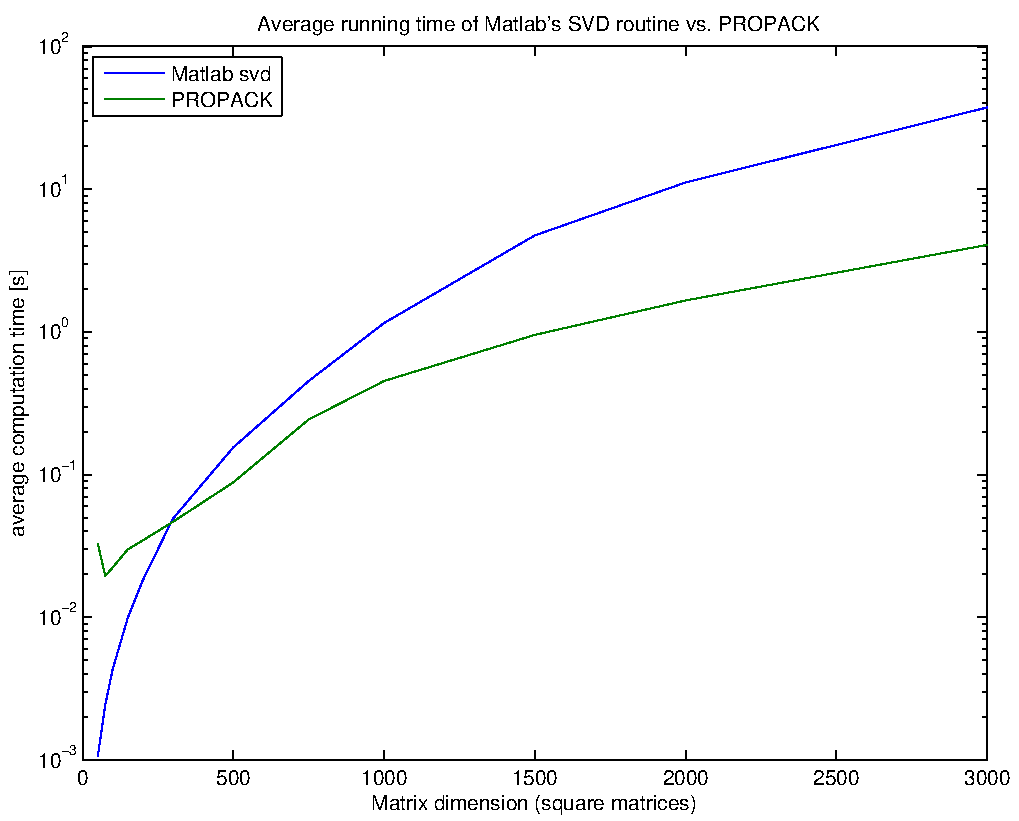
\includegraphics[width=0.75\textwidth]{../figures/svd_comparison}
\caption{Numerical comparison of Matlab's and PROPACK's SVD routines}
\label{Algorithms:Discussion:SVD:MatlabVSPropack:figure}
\end{figure}

When the matrix under consideration is sparse, the SVD can be carried out much faster using specialized methods~\cite{Berry:2005uq}. Unfortunately, while the iterates of the matrix~$S_k$ (in case of primal algorithms) are indeed sparse, the matrices for which the SVD actually needs to be computed are not. Therefore it does not seem clear how sparse SVD methods could help in improving performance of SVD-based Robust PCA algorithms. 


%%%%%%%%%%%%%%%
\subsubsection{Partial SVD methods}
\label{Algorithms:Discussion:SVD:PartialSVD:Subsubsec}

If we look at the a Singular Value Thresholding operation it is obvious that we really only needs to compute those singular values that lie above the specified threshold (which is known a priori in each step and does not depend on the singular values), since the other singular values will be set to zero anyway. One possibility to speed up the algorithms that involve thresholding of singular values is therefore to use a partial SVD to compute only those singular values of interest. For the APG algorithm the authors of~\cite{Lin:2010fk} use the software PROPACK that allows the computation of such a partial SVD. However, PROPACK by default requires the dimension of the principal singular space whose singular values are larger than the threshold, which is of course unknown a priori. Since it turns out that the rank of the the iterates~$L_k$ in the APG algorithm is monotonically increasing, a reasonable prediction of this dimension is not too hard~\cite{Lin:2010fk}. Doing so then allows to a partial SVD at each step rather than a full SVD, which can potentially speed up the algorithm (if the partial SVD can be computed efficiently). 

The PROPACK package has later also been modified to allow the computation of those singular values above a given threshold~\cite{Lin:2011kx}. Figure~\ref{Algorithms:Discussion:SVD:lasvdThrVSlasvd:figure} shows a comparison of the computation times of PROPACK's standard (full) SVD routine and the algorithm~\cite{Lin:2011kx} for different thresholds. Contrary to what one would expect, the full SVD in all cases is significantly faster than the partial SVD. At this point it is not clear what the reason for this is. Either the algorithm for performing the ``thresholded SVD'' itself is very slow, or the implementation that is provided by~\cite{Lin:2011kx} is extremely inefficient (or both). Either way, it obviously makes no sense to use to the provided implementation to compute partial SVDs. This is not to say that partial SVD is in generally slow. In fact, in~\cite{Lin:2010fk} it is found that computing the partial SVD for a fixed dimension of the principal singular space using PROPACK indeed results in a speedup of the APG algorithm. 
%
\begin{figure}[htbp]
\centering
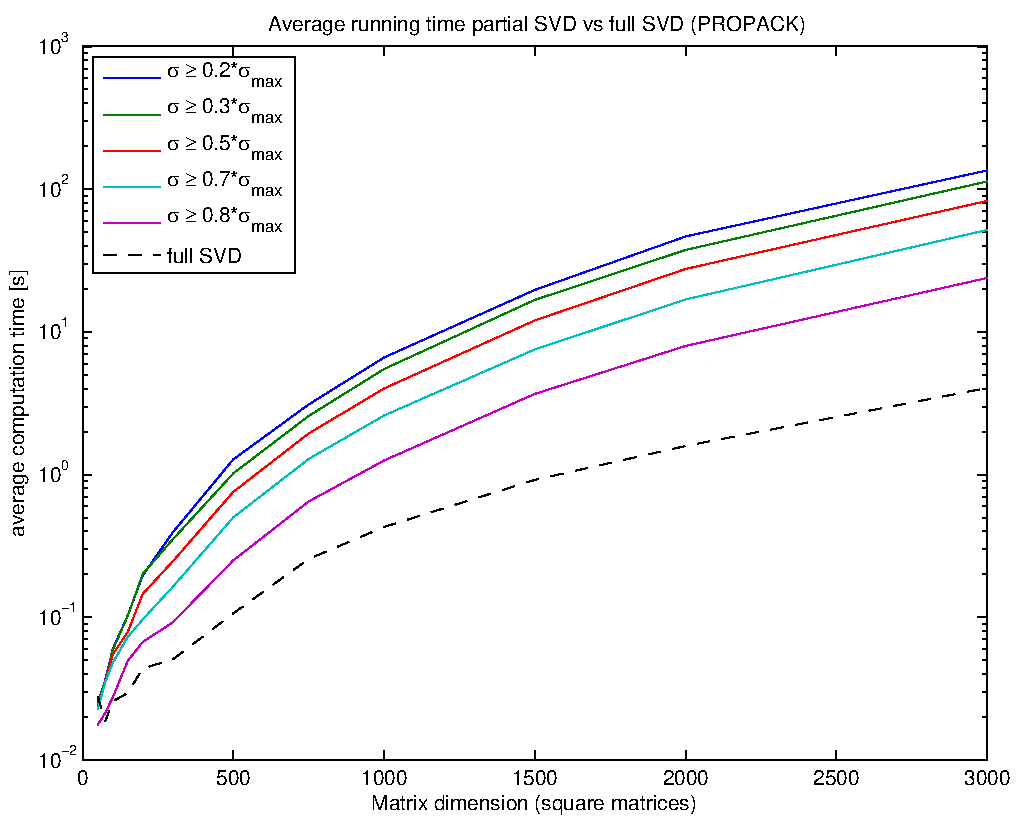
\includegraphics[width=0.75\textwidth]{../figures/thresh_svd_comparison}
\caption{Numerical comparison of partial and full SVD via PROPACK}
\label{Algorithms:Discussion:SVD:lasvdThrVSlasvd:figure}
\end{figure}

If we look at the discussed algorithms, we notice another problem with the partial SVD methods: the value of the threshold for the singular value thresholding operation in all cases decreases with the iteration number. Hence the number of singular values that need be computed actually grows with the number of iterations, which means that computing a partial SVD yields the highest benefit only in the early stages of the algorithm. 


%%%%%%%%%%%%%%%
\subsubsection{Warm-start methods for SVD}
\label{Algorithms:Discussion:SVD:WarmstartSVD:Subsubsec}

Another potential way of speeding up many SVD-based algorithms is to exploit the fact that the matrix of which the SVD has to be computed does generally not change much between iterations, in particular after a few iterations. To utilize this fact, the authors of~\cite{Lin:2010uq} propose a warm start technique for the block Lanczos method for SVD computation. In the following section we will also provide simulation results of an inexact ALM algorithm based on this warm-start SVD method. 



%%%%%%%%%%%%%%%%%%%%%%%%%%%%
\subsection{Numerical Comparison of Robust PCA algorithms}
\label{Algorithms:Discussion:NumComp:Subsec}

In this section we provide some simulation results to illustrate the performance of the different Robust PCA algorithms. As seen in section~\ref{Algorithms:MainAlgs:IPM:Complexity:Subsubsec}, using interior point methods to solve the dual problem is computationally infeasible for all but the smallest problems, hence we will not include interior point methods into the comparison. Furthermore, the iterative thresholding method, while applicable also to very large problem sizes, exhibits extremely slow convergence. For a comparable relative error the required number of iterations (and therefore the computation time) for problems of reasonable size is so large that a more detailed comparison with the faster APG and ALM algorithms seems unnecessary. 

The implementation of the algorithms used for the simulation are slightly modified versions of the matlab code that is freely available from \url{http://perception.csl.uiuc.edu/matrix-rank/sample_code.html}. The files are all provided with this report. 

All of the numerical results that will be presented in this section have ben obtained from simulations on randomly generated data. The (square) test matrices were generated as  $M=L+S$, where the low rank component $L$ was formed as $L=L_1L_2^T$, with $L_i \in \Rbb^{n\times r}$ where $r=0.1n$ is the rank of~$L$, and each entry $(L_i)_{i,j}$ i.i.d. Gaussian with variance~$\sigma^2 =n^{-1}$. The cardinality of the support of the sparse error component~$S$ was chosen as~$0.1n$, with each non-zero entry i.i.d uniform in $[-500,500]$. For each of the selected matrix dimensions between we simulated 10 different scenarios and computed the average overall running time, the average number of iterations and the average relative errors $\|L-\Lhat\|_F / \|L\|_F$ and $\|S-\Shat\|_F / \|S\|_F$. 


As can be seen from the first comparison in Figure~\ref{Algorithms:Discussion:NumComp:ALG_incDual:figure}, the Dual Projected Gradient Ascent algorithm (\texttt{dpga}) is much slower than both the Accelerated Proximal Gradient method (\texttt{apg}) and the Exact and Augmented Lagrangrian Method (\texttt{ealm}). Therefore we will exclude the Dual Projected Gradient Ascent algorithm from the following comparisons. 
%
\begin{figure}[h]
\centering
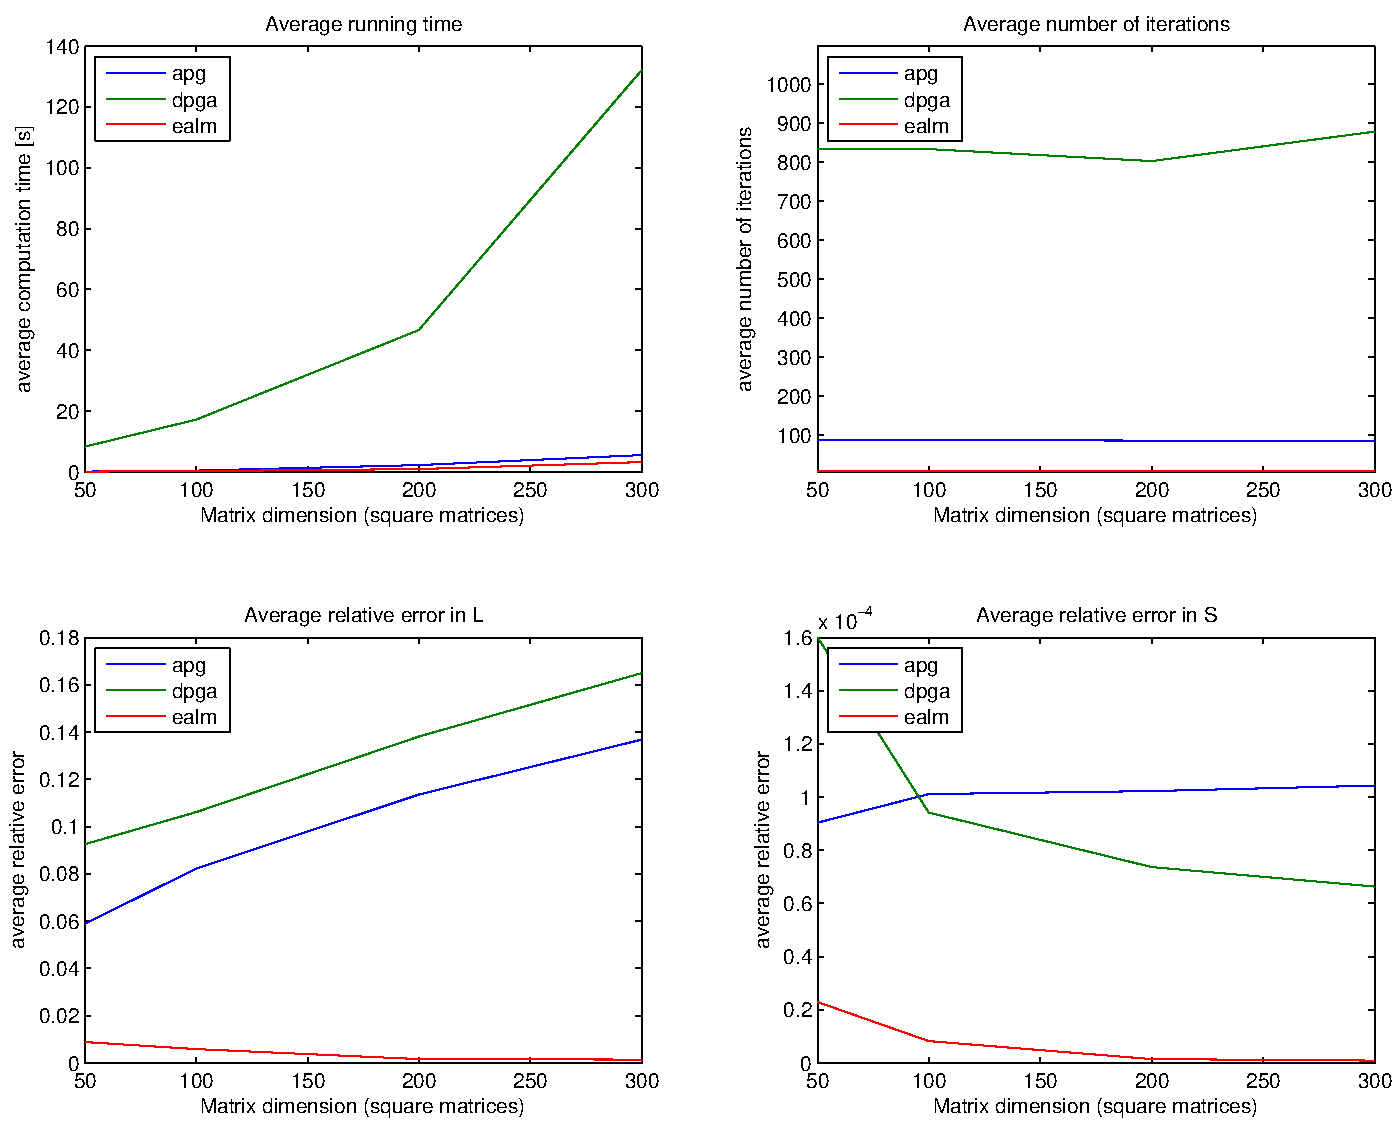
\includegraphics[width=0.95\textwidth]{../figures/ALG_comparison_incDual}
\caption{Simulation result for different algorithms for Robust PCA}
\label{Algorithms:Discussion:NumComp:ALG_incDual:figure}
\end{figure}

This leaves us with the Accelerated Proximal Gradient method (\texttt{apg}), the Accelerated Proximal Gradient method with partial SVD (\texttt{papg}), the Exact and Inexact Augmented Lagrangrian Methods (\texttt{ealm} and \texttt{ialm}, respectively) and the Inexact Augmented Lagrangrian Method with warm-start Block Lanczos SVD computation (\texttt{BLWSialm}). Figure~\ref{Algorithms:Discussion:NumComp:ALG:figure} shows simulation results for these algorithms on matrices of sizes between~$n=50$ and~$n=1500$.
%
\begin{figure}[h]
\centering
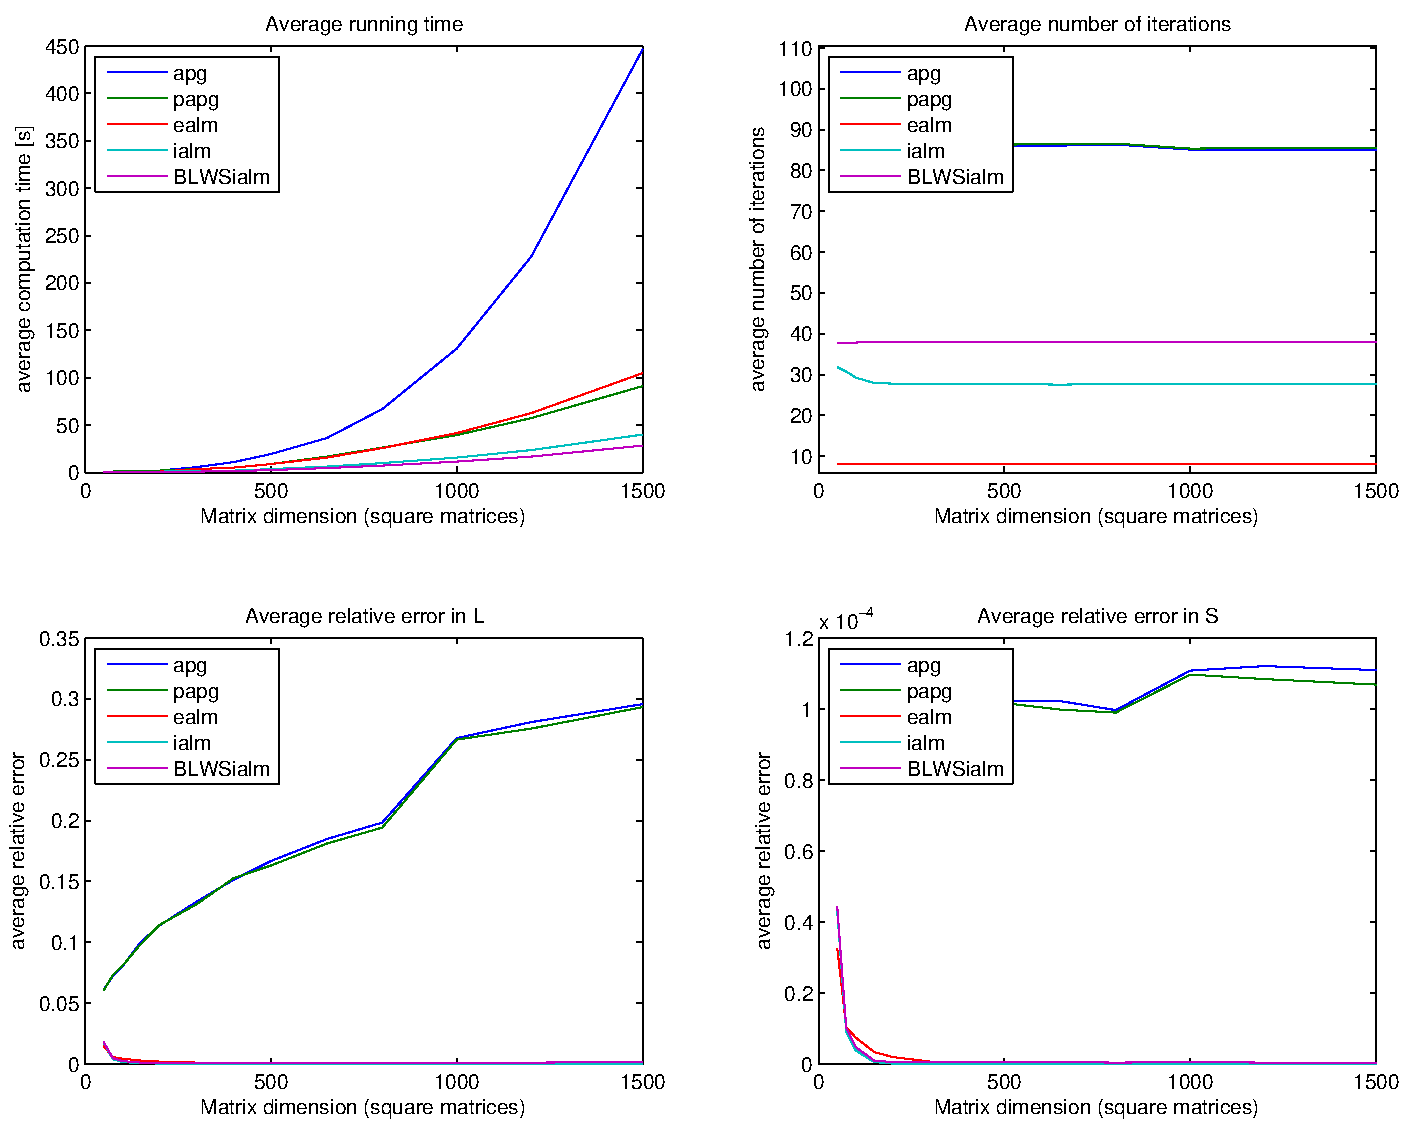
\includegraphics[width=0.95\textwidth]{../figures/ALG_comparison}
\caption{Numerical comparison of first-order algorithms for Robust PCA}
\label{Algorithms:Discussion:NumComp:ALG:figure}
\end{figure}
%

From Figure~\ref{Algorithms:Discussion:NumComp:ALG:figure} we can see that there is a clear qualitative and quantitative difference between the APG-based algorithms and the ALM-based algorithms in terms of the relative errors, with the ALM-based algorithms achieving much higher accuracies, in particular problems of large size. This relates back to Remark~\ref{Algorithms:MainAlgs:PGM:APGRPCA:AccRemark}, in which we pointed out that the APG algorithm provides only an approximate solution to the problem (to be fair, we also chose the tolerance of the APG-based algorithms a slightly higher so as to achieve comparable average running times). Moreover, we notice that the number of iterations of the APG-based algorithms is much higher than the one of the ALM-based algorithms, in particular the one of the exact ALM algorithm\footnote{note that for this algorithm we only count the outer number of iterations, not the inner iterations that are needed for solving the subproblem using the alternating directions method}. Interestingly, the number of required iterations for all of the simulated algorithms is more or less independent of the problem size. Figure~\ref{Algorithms:Discussion:NumComp:ALG:figure} also shows that the APG algorithm using partial SVD computation (\texttt{papg}) is significantly faster than the one computing a full SVD at each step (\texttt{apg}). As one would expect, the average number of iterations in both cases is the same. 


%%%%%%%%%%%%%%%
\subsubsection{Numerical Comparison of ALM-based algorithms}
\label{Algorithms:Discussion:NumComp:ALG:ALM}

The previous simulation results show that the Augmented Lagrangian Methods are superior to all other algorithms discussed so far, both in terms of average running time and in terms of accuracy (the memory requirements do not differ much between the first-order algorithms). At this point we do not see any reason to use a different algorithm, at least for the type of problem we study here. In our final simulation study, summarized in Figure~\ref{Algorithms:Discussion:NumComp:ALM:figure}, we compare the different ALM-based algorithms, namely the Exact and Inexact Augmented Lagrangrian Methods (\texttt{ealm} and \texttt{ialm}, respectively) and the Inexact Augmented Lagrangrian Method with warm-start Block Lanczos SVD computation (\texttt{BLWSialm}). We consider random (square) data matrices up to dimension $n=3000$.

Here the verdict is also quite clear, with both inexact ALM algorithms consistently faster than the exact ALM algorithm, while achieving a comparable accuracy. For all but the smallest matrix dimensions, the inexact ALM algorithm based on the warm-start Block Lanczos SVD computation is faster (about 1.5x) than the standard inexact ALM algorithm. However, its accuracy is generally lower (this can be more easily seen in Figure~\ref{Algorithms:Discussion:SVD:BLWScomptarison:figure}, which does not include the exact ALM algorithm). It should be pointed out that this is also the case when the tolerance of the stopping criterion is reduced. This seemingly counterintuitive behavior is due to the fact that the SVD computation of the warm-start Block Lanczos SVD method is inherently approximate (which is not the case for the standard inexact ALM algorithm). What is remarkable in Figure~\ref{Algorithms:Discussion:SVD:BLWScomptarison:figure} is that the number of iterations is essentially independent of the matrix size. Note however that this strong consistency very likely also has to do with the fact that all the considered randomly generated matrices are structurally identical. 

%
\begin{figure}[h]
\centering
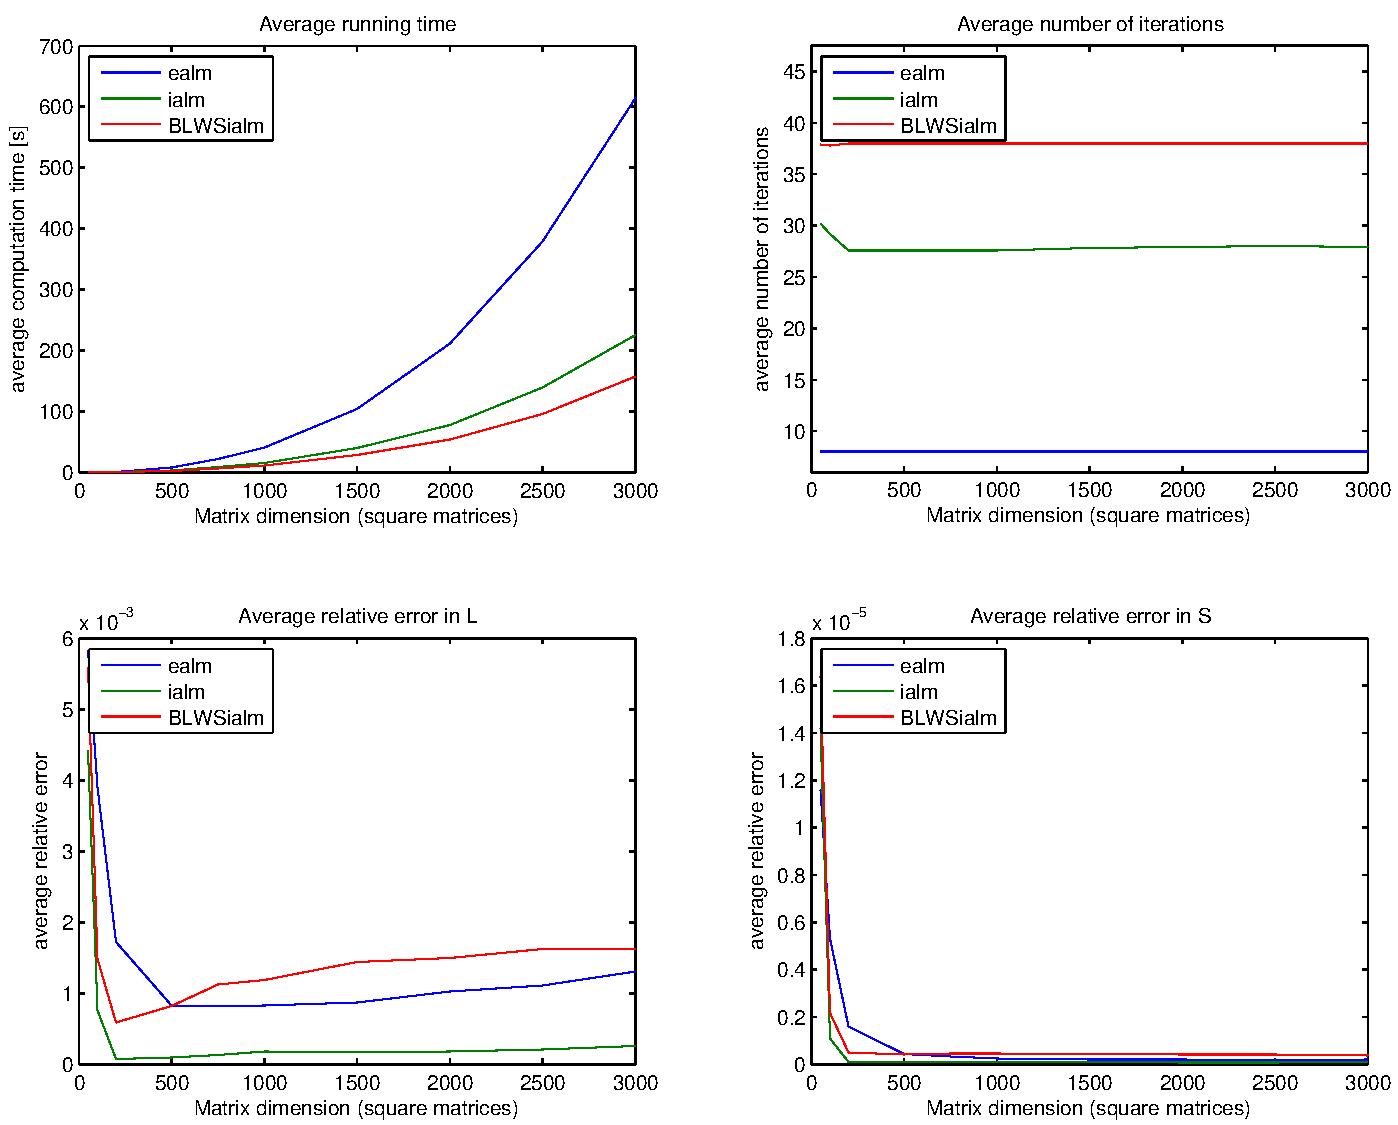
\includegraphics[width=0.95\textwidth]{../figures/ALM_comparison}
\caption{Numerical comparison of different ALM methods for Robust PCA}
\label{Algorithms:Discussion:NumComp:ALM:figure}
\end{figure}
%
%
%
%
%Figure~\ref{Algorithms:Discussion:SVD:BLWScomptarison:figure} shows a comparison of the performance of the warm-start block Lanczos method~\cite{Lin:2010uq} on synthetic data of different size. It can be seen that the running time of the warm-start method is roughly two thirds of that of the standard method, over all dimensions considered in the simulation. The relative errors of the solution, given by $\|\hat{L}-L\|_F/\norm{L}{F}{}$ and $\|\hat{S}-S\|_F/\norm{S}{F}{}$, respectively, are generally worse than those of the standard method. This is due to the fact that only an approximate SVD is computed at each iteration. What is remarkable in Figure~\ref{Algorithms:Discussion:SVD:BLWScomptarison:figure} is that the number of iterations is essentially independent of the matrix size. Note however that this strong consistency very likely also has to do with the fact that all the considered randomly generated matrices are structurally identical. 
%
%We want to emphasize here that the implementation of the warm-start block Lanczos method, as provided by~\cite{Lin:2011kx}, is completely Matlab-based and not fully optimized for performance. A careful implementation of the complete warm-start block Lanczos based inexact ALM algorithm in a performance-oriented language such as~C can be expected to yield further speedups. Nevertheless, even with the current implementation it is possible to solve rather large problems quite fast, with problems involving matrices with tens of million entries being solved in a few minutes. 

\begin{figure}[h]
\centering
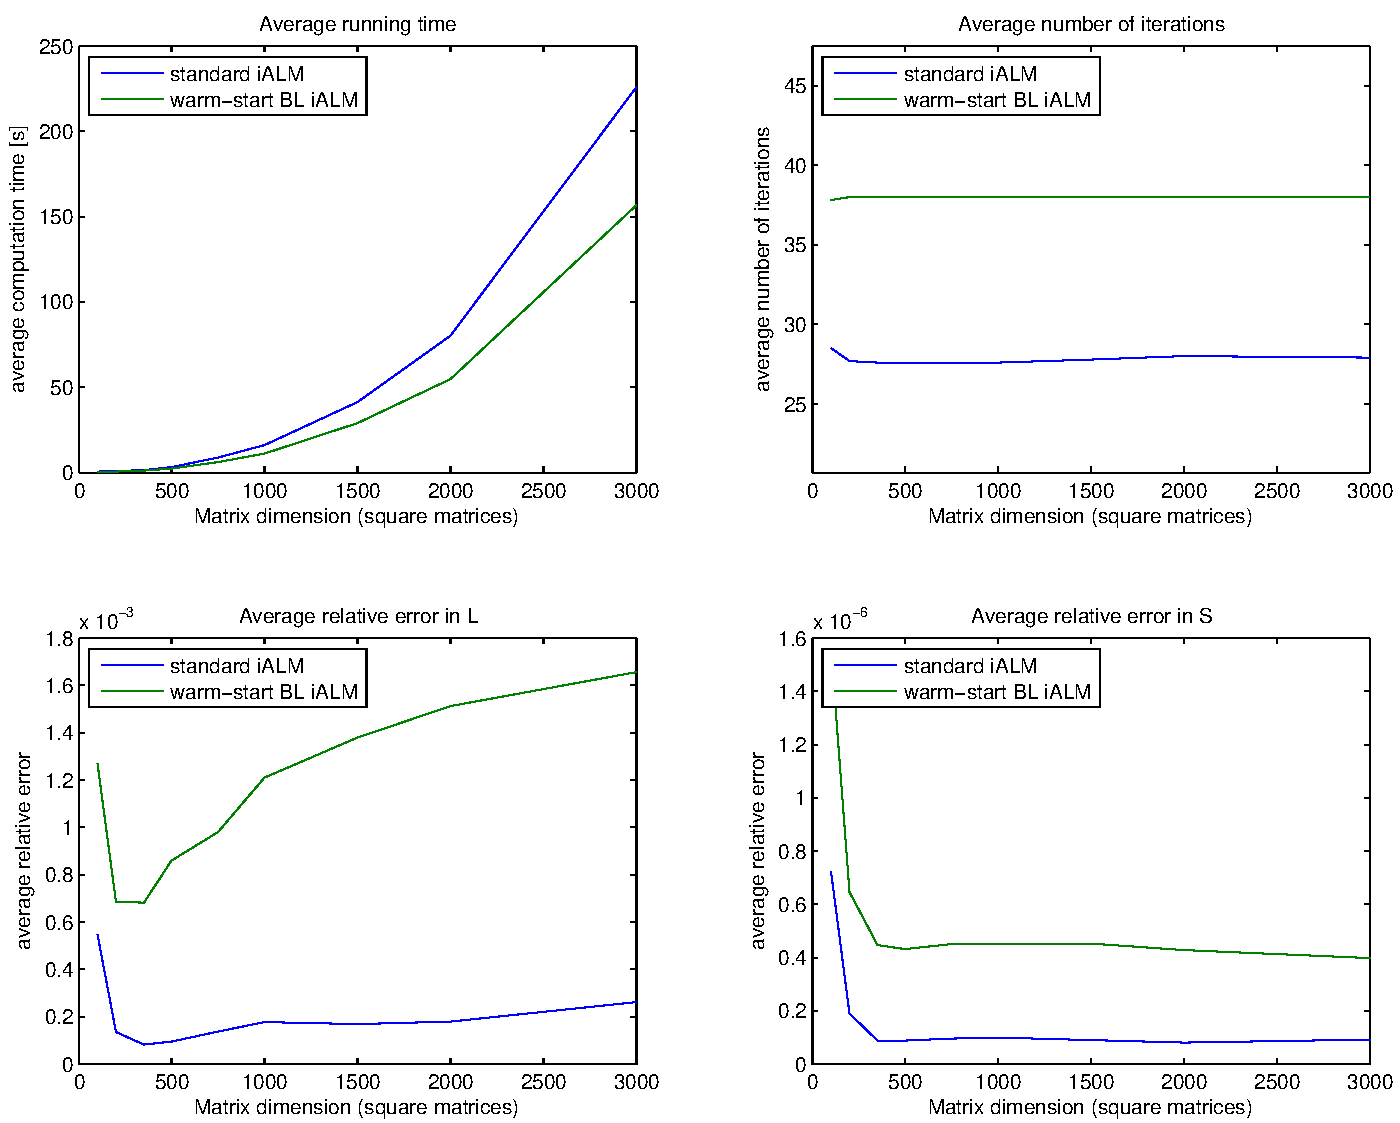
\includegraphics[width=0.95\textwidth]{../figures/BLWS_comparison}
\caption{Numerical comparison of warm-start vs. standard Block-Lanczcos method}
\label{Algorithms:Discussion:SVD:BLWScomptarison:figure}
\end{figure}

We want to emphasize here that the implementation of the warm-start block Lanczos method, as provided by~\cite{Lin:2011kx}, is completely Matlab-based and not fully optimized for performance. A careful implementation of the complete warm-start block Lanczos based inexact ALM algorithm in a performance-oriented language such as~C can be expected to yield further speedups. Nevertheless, even with the current implementation it is possible to solve rather large problems quite fast, with problems involving matrices with tens of million entries being solved in just a few minutes. 









%%%%%%%%%%%%%%%%%%%%%%%%%%%%
\subsection{Possible Directions for Parallelization}
\label{Algorithms:Discussion:Parallel:Subsec}

With the advent of highly parallelized computing architectures in modern CPUs and GPUs, a number of projects have been devoted to the development and implementation of algorithms that exploit this massive computing power. Examples for these are MAGMA~\cite{Smith:2010tg} and CULA~\cite{Humphrey:2010kl}, which are adapting classic high-performance linear algebra packages such as LAPACK and BLAS to the highly parallelized architecture of modern GPUs. 

Some of the steps in the discussed SVD-based algorithms are inherently parallelizable, for example the entry-wise soft-thresholding of a matrix, the elementary matrix operations or the computation of the Frobenius norm for the stopping criterion. The parallelization of the SVD is less obvious, but research in this area is quite active and some methods have been proposed~\cite{Berry:2005uq}. At this point we do not want to go into the details of how to parallelize the surveyed algorithms (in particular the fast augmented Lagrangian methods), we merely want to point out that we indeed see potential for further speedups and hence the use of the discussed algorithms also on large-scale data.
%
%
%\cite{Boyd:2011hc}



%%%%%%%%%%%%%%%%%%%%%%%%%%%%%%%%%%%%%%%%%%%%
\section{Outlook: Algorithms for Stable Principal Component Pursuit}
\label{Algorithms:StablePCP:Sec}

As was discussed in section~\ref{related:stablePCP}, the results obtained for the Robust PCA problem have been extended to the case when in addition to the sparse noise, the data is corrupted also by a small non-sparse noise component~\cite{Zhou:2010vn}. This problem is usually referred to as Stable Principal Component Pursuit (Stable PCP). The associated optimization problem is 
%
\begin{align}
\begin{split}
p^* = \min_{L,S} \; &\norm{L}{*}{} + \lambda \norm{S}{1}{} \\
\text{s.t.} \quad &\norm{M - L - S}{F}{} \leq \delta
\end{split}
\label{Algorithms:StablePCP:StablePCP}
\end{align}
%
where $\delta>0$ is given. In this section we want to give a brief outlook on what algorithms have been proposed for~\eqref{Algorithms:StablePCP:StablePCP}. While to date the literature on algorithms for this problem is less extensive than for the classic Robust PCA problem, a number of efficient ALM algorithms have already been proposed. 

First of all, it is not hard to reformulate problem~\eqref{Algorithms:StablePCP:StablePCP} as an SDP, which can then in principle be solved using general purpose interior point solvers. However, the same scalability issues as in the standard Robust PCA problem will prohibit the use of these methods for most problems of practical interest.

In the original Stable PCP paper~\cite{Zhou:2010vn}, the authors directly use the Accelerated Proximal Gradient (APG) algorithm from section~\ref{Algorithms:MainAlgs:PGM:APGRPCA:Subsubsec} for solving an approximate version of~\eqref{Algorithms:StablePCP:StablePCP}. Using a duality argument it is easy to see that~\eqref{Algorithms:StablePCP:StablePCP} is equivalent to
\begin{align*}
\min_{L,S} \; &||L||_* + \lambda ||S||_1 + \frac{1}{2\mu} ||M-L-S||_F
\end{align*}
for some value~$\mu(\delta)$. Note that the above problem is just~\eqref{Algorithms:MainAlgs:PGM:APGRPCA:Relax}. The authors make the argument that it makes sense to choose $\mu$ to be the smallest value such that the minimizer of is likely to be $\Lhat = \Shat = 0$ if $L=S=0$ and $M=Z$. In this way, $\mu$ is large enough to threshold away the noise, but not too large to over-shrink the original matrices. Assuming an iid Gaussian distribution of the dense noise component, i.e. $(Z_0)_i,j) \sim \Ncal(0,\sigma^2)$, it turns out\footnote{this based on the strong Bai Yin Theorem~\cite{Bai:1988fk}, which implies that for an $n\times n$ real matrix with entries $\xi_{ij} \sim \Ncal(0,1)$ the it holds that $\limsup_{n\rightarrow \infty} \norm{Z_0}{2}{}/\sqrt{n} = 2$ almost surely} that $n^{-1/2}\norm{Z_0}{}{} \rightarrow \sqrt{2} \sigma$ a.s. as $n\rightarrow \infty$. As a result of this, the choice for~$\mu$ becomes~$\mu = \sqrt{2n}\sigma$. We note that the assumption of a Gaussian noise matrix~$Z_0$ is often reasonable but not always satisfied. If it is not, then it is not clear whether using the APG algorithm to solve the associated approximate problem is a good idea and different algorithms may be needed. 


In~\cite{Tao:2011vn} an algorithm for~\eqref{Algorithms:StablePCP:StablePCP} based on partial variable splitting is proposed\footnote{The authors in fact consider the more general problem where the constraint reads $\norm{\Pcal_\Omega (M - L - S)}{F}{} \leq \delta$, where $\Pcal_\Omega$ is the projection on the set~$\Omega$ of observed data}. In fact, the problem an simply be written as 
%
\begin{align}
\begin{split}
p^* = \min_{L,S,Z} \; &\norm{L}{*}{} + \lambda \norm{S}{1}{} \\
\text{s.t.} \quad & M = L +  S + Z \\
&\norm{Z}{F}{} \leq \delta
\end{split}
\label{Algorithms:StablePCP:PartialVarSplitting}
\end{align}
%
At heart, the proposed ASALM algorithm is the extension of the ALM method from section~\ref{Algorithms:MainAlgs:AugLag:RPCA:Subsubsec} to the case with partial variable splitting. It turns out that the additional subproblem appearing at each iteration can be solved explicitly at a cost similar to the matrix value thresholding (the cost of which is~$O(mn)$). The dominant computation is still the singular value thresholding operation that is based on the computation of the SVD. Hence the proposed method is comparable in computational complexity to the ALM method from section~\ref{Algorithms:MainAlgs:AugLag:RPCA:Subsubsec}.

In~\cite{Aybat:2011vn} a number of different algorithms for Stable PCP are discussed, most of which are based on a smoothed or partially smoothed objective function. Two of these algorithms essentially apply Nesterov's optimal algorithms~\cite{Nesterov:2005fk} to the partially smoothed problem, which yields a theoretical complexity of~$O(1/\varepsilon)$. It is further shown that the subproblems appearing in these algorithms either have a closed-form solution or can be solved very efficiently. Still using a partially smoothed objective function, the authors also apply a partial variable splitting technique and propose to use an alternating minimization algorithm for a linearized version of the associated augmented Lagrangian function. This also yields an algorithm with a theoretical complexity of~$O(1/\varepsilon)$. 

The authors of~\cite{Aybat:2011vn} also propose a first-order algorithm that works directly with the fully non-smooth objective, which they call NSA. Very similar in nature to the ASALM method proposed in~\cite{Tao:2011vn}, this algorithm is also an extension of the ALM method from section~\ref{Algorithms:MainAlgs:AugLag:RPCA:Subsubsec} to the setting with partial variable splitting. While the authors were not able to derive theoretical complexity results, empirical evidence suggests that this algorithm is quite efficient in solving the Stable PCP problem. In particular, numerical simulations indicate that NSA consistently outperforms ASALM. The main reason for this seems to be that while ASALM performs an alternating minimization over three directions ($L$, $S$ and $Z$), NSA uses the fact that the joint minimization over $(S,Z)$ also has an explicit solution and therefore only alternates over two directions. 


%%%%%%%%%%%%%%%%%%%%%%%%%%%%%%%%%%%%%%%%%%%%%%%%%%%%%%%%%%%%%%%%%%%%
%\bibliographystyle{abbrv}
%\bibliography{../../common/RobustPCA}


%%%%%%%%%%%%%%%%%%%%%%%%%%%%%%%%%%%%%%%%%%%%%%%%%%%%%%%%%%%%%%%%%%%%
%\end{document}  

